% !TeX root = ../thesis.tex
\chapter{Grundlagen}
\label{chap:fundamentals_related-work}
In diesem Kapitel werden die Grundlagen eines modernen Übertragungssystems vorgestellt. Da eine Audioübertragung mittels \gls{acr:VLC}-Technik implementiert werden soll, wird zunächst auf die Eigenschaften eines zu Übertragenden Audiosignals eingegangen. Darauf folgend werden einige Grundlagen zur Übertragungstechnik und der verwendeten elektronischen Bauteile erläutert. Hier werden grundlegende Funktionsweisen sowie deren Rolle in der analogen und digitalen Signalverarbeitung thematisiert. 

\section{Audio}
\label{subsec:Unterabschnitt1}

Ziel der vorliegenden Abschlussarbeit ist die Übertragung eines Echtzeit-Audio-Signals mithilfe des projektierten \gls{acr:VLC}-Senders. Deshalb soll im nachfolgenden Kapitel anfänglich im Allgemeinen auf die Übertragung von Audiosignalen eingegangen werden. Praktische Beispiele zur Übertragung von Audiosignalen über größere Entfernung ergeben sich bei der Übertagung von Sprache und Musik. Hierbei wird zunächst der Hörschall mit Hilfe eines Mikrofon in ein proportionales elektrisches Signal umgewandelt. Dieses Signal wird anschließend auf drahtlosem oder drahtgebundenem Wege dem Empfänger übermittelt. Ein gängiges Beispiel für die drahtlose Übertragung ist die Rundfunkübertragung. Mit Telefon und Kabelrundfunk ergeben sich Beispiele für eine drahtgebundene Übertragung. Häufig kommt jedoch eine Kombination aus beidem zum Einsatz. Am Empfangsort wird das elektrische Signal mittels eines Wiedergabegerätes, wie zum Beispiel einem Lautsprecher, wieder in ein akustisches Signal überführt.

Der, durch den Lautsprecher entstandene, hörbare Schall besteht aus einer mechanischen Welle. Diese ist definiert durch eine Frequenz, welche die Tonlage bestimmt und einer Amplitude, die in diesem Fall die Lautstärke des Audiosignals vorgibt. Damit sich die Welle im Raum ausbreiten kann, um zum Empfänger zu gelangen, benötigt sie ein Übertragungsmedium. Die Dichte eines Mediums bestimmt die Geschwindigkeit, in der sich die Welle ausbreitet. Je dichter das Medium ist, desto schneller kann sich eine Welle ausbreiten.

Trifft die sich ausbreitende mechanische Welle auf das menschliche Trommelfell, wird dieses in Schwingung versetzt und regt somit die menschlichen Nerven an. Das Signal wird an dieser Stelle von einer mechanischen Welle in ein elektrisches Signal gewandelt, das über die Nervenbahnen zum Gehirn weitergeleitet wird. Im Gehirn wird das elektrische Signal analysiert und mit semantischen Informationen verbunden, die das Hören ermöglichen. Ob ein Ton von einem Menschen wahrgenommen werden kann, hängt einerseits von der Frequenz und der Amplitude des Audiosignals ab und anderseits von der wahrnehmenden Person. So gibt es nur einen bestimmten Bereich von Frequenzen der von einem Menschen wahrgenommen werden kann. Frequenzen unterhalb des menschlichen Hörbereichs werden Infraschall genannt, darüber liegende Frequenzen werden als Ultraschall bezeichnet (siehe Abbildung 2.1). Die Grenzen dieses Hörbereiches sind nicht nur von Mensch zu Mensch unterschiedlich, sondern verschieben sich auch mit zunehmendem Alter. Daher kann der Frequenzbereich des menschlichen Hörens nicht einheitlich bestimmt werden. Dies erklärt warum zum Teil unterschiedliche Angaben in der Literatur zu finden sind. Plassmann gibt den Hörbereich zwischen 16 Hz und 16 kHz an [Pla16]. Stotz hingegen zwischen 20 Hz bis 20 kHz [Sto11]. Der hörbare Frequenzbereich eines menschlichen Ohres unterscheidet sich hingegen stark von zum Beispiel dem eines Hundes. Hunde haben ein viel feineres Gehör als Menschen. Ihr Hörbereich reicht von 65 Hz bis 45 kHz .
\begin{figure}[H]
	\centering
	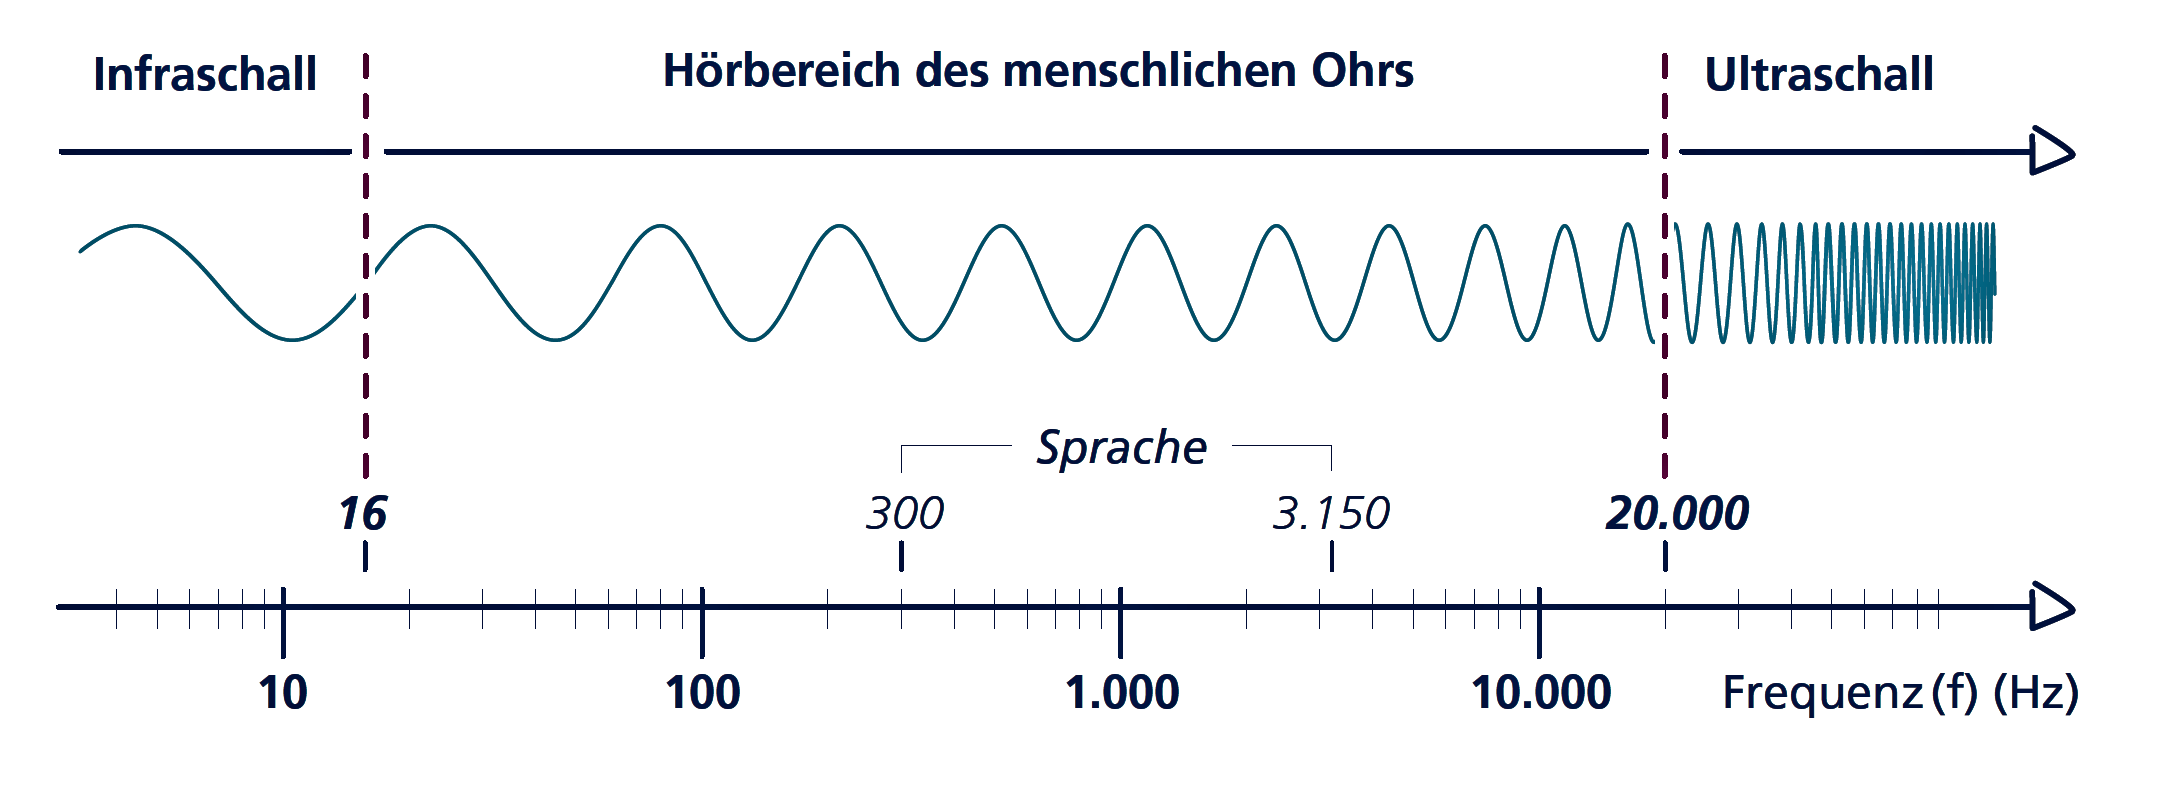
\includegraphics[width=1\textwidth]{audiospektrum.png}
	\caption[Hörbereich des menschlichen Ohres]{Hörbereich des menschlichen Ohres} \cite{michelsSonographieOrganUnd2012}
	\label{fig:audiospektrum}
\end{figure}
Neben dem beschreiben Hörbereich beeinflusst auch der Abstand zu einer Quelle die Wahrnehmung des Signals. Durch Freiraumdämpfung verringert sich die Amplitude einer sich
ausbreitenden Welle, mit zunehmende Distanz wodurch die Lautstärke abnimmt. Befinden
sich eine Quelle außerhalb der Hörreichweite, werden häufig analoge oder digitale Kommunikationssysteme verwendet, um eine Übertragung zu ermöglichen. Zur Übertragung und Weiterverarbeitung der beschriebenen mechanischen Welle, muss diese zunächst in eine elektrische Größe gewandelt werden.
Für diese Wandlung wird für Audiosignale ein Mikrofon verwendet. Ähnliche wie es mit dem Trommelfell im menschlichen Ohr passiert, wird im Inneren des Mikrofons eine Membran in Schwingung versetzt und erzeugt hierdurch eine elektrische analoge Spannung.
Zur digitalen Verarbeitung des Signals muss dieses mithilfe eines Analog-Digital-Wandlers
(AD-Wandler) in digitale Werte gewandelt werden. Hierfür wird die Analogspannung in zeitlich regelmäßigen (äquidistanten) Abständen ausgewertet und abgespeichert. Dieser
Vorgang wird Abtastung genannt. Wie in Abbildung 2.2 zu sehen, entstehen einzelne
Impulse mit Werten des Signals. Zwischen den Abtastzeitpunkten wird jedoch keine Information abgefragt, hierdurch ist der Wert an diesen Stellen Null. Um das Originalsignal zu
rekonstruieren, müssen durch einen Digital-Analog Wandler (DA-Wandler) die fehlenden Signalabschnitte interpoliert werden. Hierbei ist auf den Zusammenhang zwischen Abtastfrequenz und Signalfrequenz zu achten.


\begin{figure}[H]
	\centering
	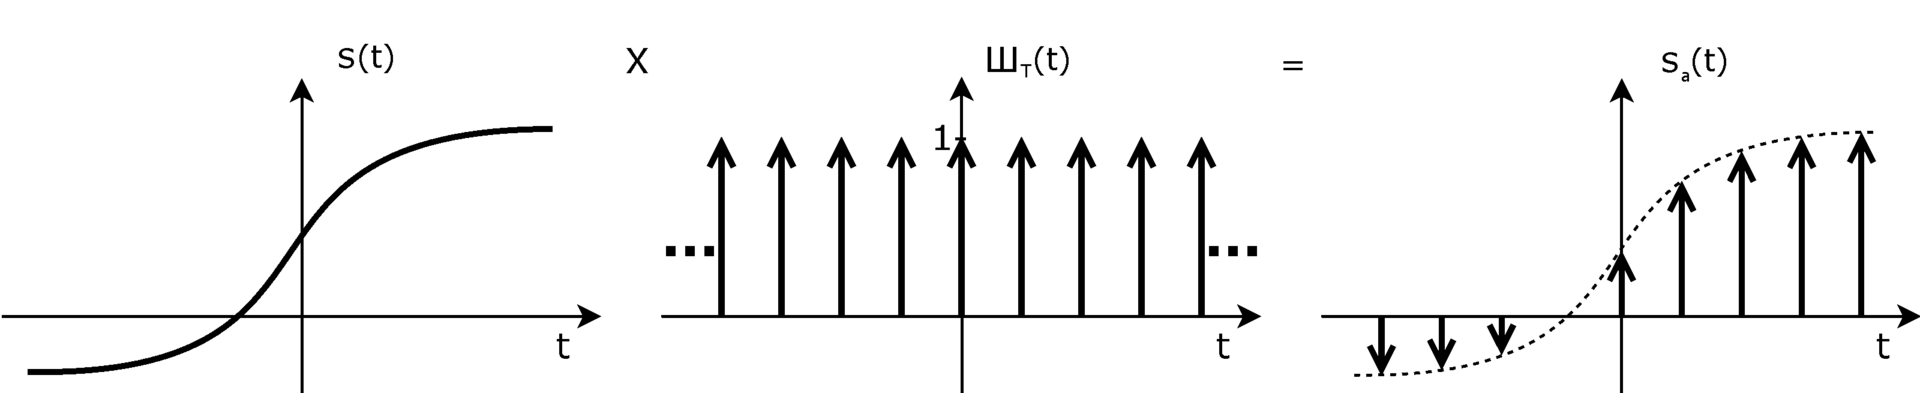
\includegraphics[width=1\textwidth]{abtastung.png}
	\caption[Abtastung eines Signals]{Abtastung eines Signals} \cite{michelsSonographieOrganUnd2012}
	\label{fig:abtastung}
\end{figure}

In Abbildung 2.2 ist zu erkennen, dass ausreichend viele Abtastwerte vorhanden sind,
um den Verlauf des Signals detailliert wiederzugeben. Die gewählte Abtastfrequenz steht
demnach in einem adäquaten Verhältnis zur Signalfrequenz. Mit einer sinkenden Anzahl
von Abtastwerten vergrößern sich die Signallücken, wodurch die Rekonstruktion über den Analog-Digital Wandler (AD-Wandler) zunehmend erschwert wird. Nach dem Theorem von Shannon ist für die höchste Signalfrequenz pro Schwingung mindestens eine zweimalige Abtastung erforderlich, um das Signal perfekt rekonstruieren zu können. Hierbei gilt also:

\begin{equation}
	\label{equ:bsp1}
	F_{A} \geq 2 \cdot F_{S}
\end{equation}

Wobei $F_{A}$ fur die Abtastfrequenz und $F_{S}$ fur die höchste im Signal enthaltende Frequenz
steht. In Abbildung 2.3 befolgt die obere Abtastung die Regel von Shannon, während die unter sie verletzt. Wie zu erkennen ist, gelingt durch die richtige Abtastung eine gute Rekonstruktion, während bei Unterabtastung das Signal stark verfälscht rekonstruiert wird.

\begin{figure}[H]
	\centering
	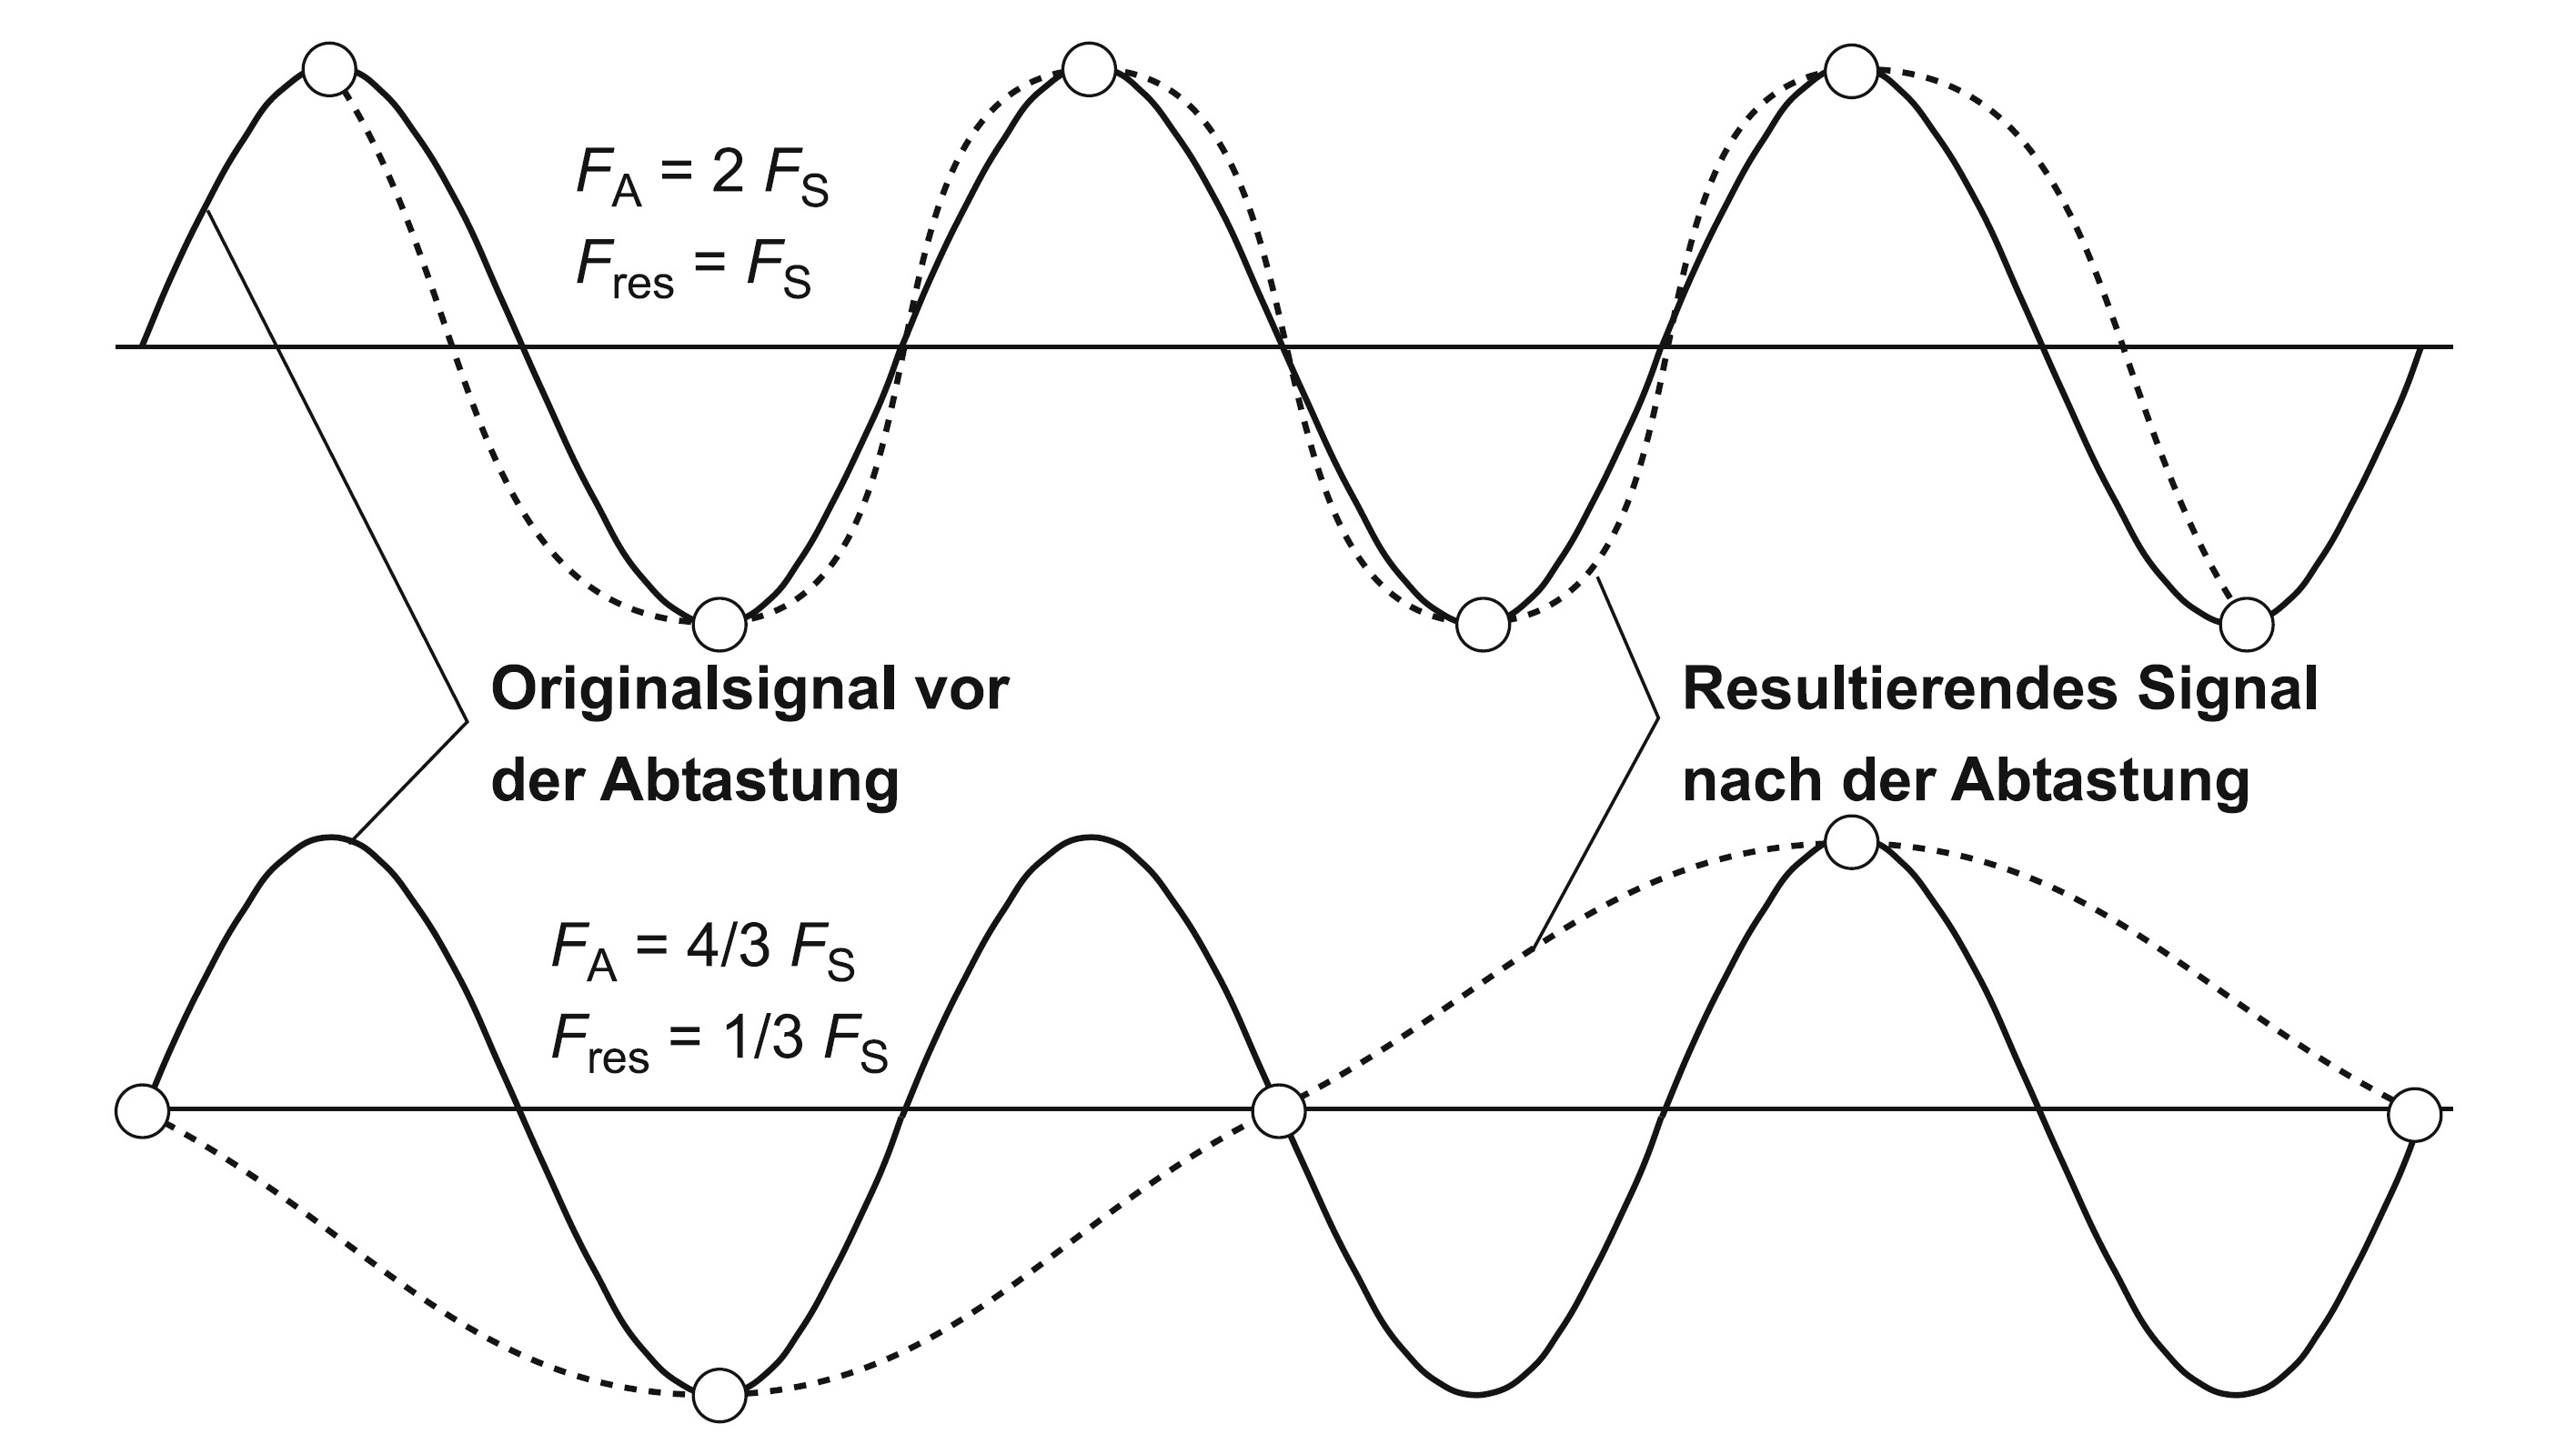
\includegraphics[width=0.8 \textwidth]{shannon.jpg}
	\caption[Unterabtastung eines Signals]{Unterabtastung eines Signals} \cite{stotzComputergestuetzteAudioUnd2019}
	\label{fig:shannon}
\end{figure}

Des Weiteren ist zu erkennen, dass die obere Abtastung das Signal jeweils in seinen Minima
bzw. Maxima erfasst. Bei einer Phasenverschiebung von $90^\circ$ wurde die obere Abtastung jedoch genau die Nulldurchgänge des Signals erfassen. Eine Rekonstruktion des Signals wäre dann nicht mehr möglich, da es nicht mehr von einem Nullsignal unterscheidbar wäre. Aus diesem Grund ist es zu empfehlen, die Abtastfrequenz mehr als doppelt so groß, wie die größte im Signal auftretenden Frequenz f, zu wählen. Da das menschliche Gehör Töne, die oberhalb einer Frequenz von 20 kHz liegen, nicht mehr wahrnehmen kann, wird im Audiobereich meistens mit 44,1 kHz oder mit 48 kHz abgetastet und somit das
Shannon-Theorem eingehalten.\cite{stotzComputergestuetzteAudioUnd2019}




\section{Übertragungstechnik}
\label{subsec:Unterabschnitt1}

In diesem Kapitel werden die Grundlagen der modernen Übertragungstechnik als Grundlage für die weiteren Ausführungen erklärt. Zunächst soll der generelle Aufbau eines Übertragungssystems erläutert werden, um im Folgenden einige gängige digitale Modulationsarten vorzustellen.
Hierbei liegt der Fokus besonders auf einer Quadrature Phase Shift Keying (QPSK)-
Modulation, welche in den später gezeigten Modellen Verwendung findet. Der letzte Abschnitt beschäftigt sich mit den Themen Bandbreitennutzung und Mehrkanalzugriff. Hier werden die aus der Mobilfunktechnik bekannten Begriffe Frequenzmultiplexverfahren (Frequency Division-Multiple-Access) (FDMA), Zeitmultiplexverfahren (Time-Division-Multiple-Access)
(TDMA) und Codemultiplexverfahren (Code-Division-Multiple-Access) (CDMA) eingefuhrt und beschrieben.


\subsection{Aufbau eines Übertragungssystems}
\label{subsec:Unterabschnitt1}

Ein Übertragungssystem besteht stark vereinfacht dargestellt aus fünf verschiedenen Teilen. In Abbildung 2.4 ist eine Skizze eines solchen Übertragungssystems zu sehen, die im Folgenden näher beschrieben werden soll. Zunächst wird eine Quelle benötigt, welche ein zeitkontinuierliches Signal (z.B. Sprache, Musik, Bilddaten, analoge Messwerte) oder ein zeitdiskretes Signal (z.B. Buchstaben, Datensequenzen, abgetastete analoge Signale) zur Verfügung stellt. Der Sender übernimmt im System die Aufgabe, das Quellensignal in ein für die Übertragung geeignetes Format umzuwandeln. Dieses muss auf den später zur Weiterleitung des Signals genutzten Kanal abgestimmt werden. Dabei gilt es darauf zu achten, den zur Verfügung stehenden Kanal und seine Eigenschaften möglichst effizient zu nutzen. Hierbei
wird zwischen drahtlosen Kanälen (elektromagnetisch, akustisch, Infrarot) und drahtgebundenen Kanälen wie beispielsweise Kupferleitungen oder Glasfaserkabeln unterschieden.
Nach der Umwandlung des Originalsignals durch den Sender wird dieses über einen dieser physikalischen Kanäle gesendet. Ein Übertragungskanal ist im Allgemeinen fehlerbehaftet. Dies hat zur Folge, dass das Signal bei der Ausbreitung durch den Kanal verzerrt oder gedämpft wird. Es kann zudem zu Interferenzen mit anderen Kanälen oder Umwelteinflüssen kommen, welche das Übertragene Signal verfälschen.
Die Aufgabe des Empfängers besteht in einer möglichst genauen Rekonstruktion des Quellensignals. Das reproduzierte Quellensignal gelangt schließlich an die Senke. Zum Eliminieren der im Kanal entstandenen Fehler wird dem übertragenen Signal durch verschiedene Verfahren Redundanz hinzugefügt. Die angefügte Redundanz enthält keinen Informationswert, sondern dient zur Absicherung der übertragenen Daten. Der Empfänger kann durch die Redundanz Fehler erkennen und im Optimalfall auch direkt korrigieren. Näheres hierzu wird im Kapitel 2.5 erklärt.

Nach dieser allgemeinen Darstellung des Übertragungssystems soll nun eine genauere Beschreibung der Übertragungsstrecke folgen. Diese wird sich aufgrund des Schwerpunkts dieser Abschlussarbeit auf die Übertragung durch einen drahtlosen Kanal fokussieren. Zum Aufbau eines drahtlosen Übertragungssystems muss zunächst der physikalische Kanal über welchen sich das Signal ausbreitet definiert, sowie die Signalform festgelegt werden. So verwenden Fernbedienungen im Bereich der Unterhaltungselektronik beispielsweise als Signalform Licht im Infrarot-Bereich, um Daten zu Übermitteln. Hierfür muss jedoch der direkte Einfall des Lichts auf den Empfänger gegeben sein, wodurch die Reichweite dieser Art der
Datenübertragung stark begrenzt ist und sich daher nicht für andere Anwendungsgebiete wie beispielsweise den Mobilfunk eignet. Für Mobilfunkanwendungen werden in der Regel elektromagnetische Wellen im Megaherz bis Gigaherz Frequenzbereichen verwendet. Diese Wellen bestehen aus einem elektrischen und einem magnetischen Feld, wobei die beiden Felder sich orthogonal zueinander ausbreiten.
In Abbildung 2.5 ist die Ausbreitung einer solchen Welle veranschaulicht. Diese Art von
Welle ist nicht auf ein Ausbreitungsmedium angewiesen und kann sich somit auch im
Vakuum (z.B. im Weltraum) ausbreiten. Somit ermöglicht sie auch eine Kommunikation
mit Satelliten. [But13] [An19]

Zur Erzeugung einer elektromagnetischen Welle wird zunächst eine hochfrequente Wechselspannung benötigt. Diese wird meist durch einen Quarzoszillator erzeugt. Damit sich
die Welle nun ausbreiten kann, benötigt sie eine Antenne von welcher sie sich ablösen kann.
Eine elektromagnetische Welle kann sich jedoch erst dann von einer Sendeantenne lösen,
wenn die Wellenlänge $\lambda$ in die Größenordnung der Antennenabmessung kommt [Fis10]. Es
gilt:
\begin{equation}
	\label{equ:bsp1}
	\lambda = \frac{c}{f} 
\end{equation}
Ein Audiosignal erstreckt sich über einen Bereich von 20Hz bis 20kHz, wodurch nach dieser Formel eine extrem große Antenne benötigt werden wurde. Hieraus ergibt sich auch die Notwendigkeit eine geeignete, d.h. im richtigen Frequenz-, also Wellenlängenbereich
liegende Sende-, bzw. Trägerfrequenz zu wählen und die zu versendende Information dieser
durch Modulation aufzuprägen.[Höh13]

\subsection{Modulationsarten}
\label{subsec:Unterabschnitt1}

In Kapitel 2.2.1 wurde beschrieben wie ein Übertragungssystem aufgebaut ist und aus welchen Komponenten es besteht. Es wurde auch gezeigt wie eine Welle entsteht und diese sich ausbreitet. Des Weiteren wurde die Notwendigkeit einer hochfrequenten Trägerfrequenz verdeutlicht. Im nächsten Schritt soll nun gezeigt werden, wie der Trägerwelle die geforderte Information aufgeprägt wird. Hierfür stehen die drei Parameter zur Verfügung, welche eine Welle beschreiben. Dies sind die Frequenz, die Amplitude sowie die Phase der Welle. Dabei wird die Variation der Amplitude als Amplitudenmodulation (AM) oder auch
Amplitude Shift Keying (ASK) bezeichnet, eine Variation der Phase als Phasenmodulation
(PM) oder auch Phase Shift Keying (PSK) sowie die Variation der Frequenz als Frequenzmodulation (FM) oder auch Frequency Shift Keying (FSK). Im Folgenden wird erläutert,
wie diese Parameter verändert werden können, um der Welle die Information einzuprägen.
Zunächst soll die analoge Modulation anhand eines AM-Signals und eines FM-Signals gezeigt werden. Hierbei wird das analoge Ausgangssignal nicht digital gewandelt, sondern
unabgetastet verarbeitet. Bei der Amplitudenmodulation wird das zu übertragende Signal mithilfe eines Mischers, mit einer sinusförmigen Trägerfrequenz multipliziert. Das Blockschaltbild eines solchen Mischers ist in Abbildung 2.6 zu sehen.
Die deutlich langsamere Frequenz des übertragenen Signals bestimmt die Amplitude der hochfrequenten Trägerfrequenz und wird deshalb Einhüllende genannt. In Abbildung 2.7 ist gut zu erkennen, wie die Amplitude der Trägerfrequenz des AM -Signals dem Signalverlauf des Eingangsignals folgt. Das Signal hat nun eine ausreichend hohe Trägerfrequenz, welche sich von einer Antenne lösen und ausbreiten kann[Fis10]. Dem Empfänger ist es wiederum möglich, durch eine Filterung mit einem Tiefpassfilter die zuvor eingefügten hohen Frequenzanteile herauszufiltern und so das Originalsignal zu reproduzieren. Zu Problemen kann es kommen, wenn sich der Empfänger bewegt. Durch diese Bewegung variiert
die Ausbreitungsstrecke, was durch die Freiraumdämpfung zu einer Signalabschwächung
bzw. Signalstärkung fuhren kann. Bei einer Audioübertragung würde dann die Lautstärke schwanken. Im Gegensatz zu einer Amplitudenmodulation liegt bei einer Frequenzmodulation die Information nicht in der Amplitude des empfangenen Signals sondern in dessen Frequenz. Wie in Abbildung 2.7 zu sehen, verändert sich bei dem frequenzmodulierten Signal lediglich die Trägerfrequenz, nicht aber die Amplitude. Hierdurch ist diese Art der Modulation störresistenter gegenüber Amplitudenschwankungen. Allerdings können auch hier Effekte wie der Dopplereffekt das Signal beeinflussen, wenn sich Sender oder Empfänger bewegen.[Höh13]


Im Folgenden sollen nun die Grundlagen digitaler Modulationsverfahren dargestellt werden. Wie bei einer analogen Modulation, nutzen auch digitale Modulationsverfahren die Veränderung von Frequenz, Amplitude und Phase des Trägersignals. Als eine der ersten digitalen Übertragungsarten wird heute die ¨ Übertragung von Telegrammen angesehen. Hierbei wurde eine Gleichspannung aus und ein geschaltet. Ein langes Einschalten stand dabei für eine Eins, ein kurzes Einschalten für eine Null. Da diese Übertragung anfänglich noch drahtgebundenen stattfand, wurde keine Trägerfrequenz benötigt. Auf der Empfängerseite brachte die Gleichspannung eine Lampe zum leuchten oder lies ein akustisches Signal
erklingen. Je nach Länge des Einschaltens konnte somit eine Null oder eine Eins erkannt
werden.[Fis10] Aufgrund der Limitierung dieses binären Systems musste die Nachricht im
Vorfeld kodiert werden. Hierfür wurde das Morsealphabet verwendet. Um die Länge der
übertragenen Nachrichten möglichst kurz zu halten, wurde hierbei bereits versucht, eine
Redundanzreduktion zu erzeugen. Kurze Codes wurden für Buchstaben des Alphabets verwendet, die gehäuft im Sprachgebrauch auftreten, lange Codes wurden für Buchstaben verwendet, die sich weniger häufig in der Sprache wiederfinden.[Fis10] Diese Grundlage werden bis heute in der modernen Signalübertragung angewandt. In Abbildung 2.8 sind die drei digitalen Grundmodulationsarten AM, FM und PM dargestellt. Hierbei entspricht der Verlauf von Kennlinie (b) einem AM-Signal, Kennlinie (c)
zeigt ein FM-Signal und in (d) ist eine Phasenmodulation zu sehen. Das dargestellte AM Signal hat bei der Übertragung einer 1 eine definierte Amplitude und bei der Übertragung
einer 0 wird die Amplitude auf Null gesetzt. Da so nicht erkannt werden kann ob bei
ausbleibender Amplitude die Übertragung beendet ist oder einfach nur mehrere Nullen übertragen werden, wird häufig der digitalen Null ein zweiter definierter Amplitudenwert zugeordnet. So entspricht beispielsweise 1V Amplitude einer digitalen Eins und 0,5V Amplitude einer digitalen Null. Die verschiedenen übertragenen Amplituden werden auch Symbole genannt. Die hier gezeigten Modulationsarten sind zweiwertige Modulationen. Ein übertragenes Symbol entspricht auch immer einem Bit digitale Information. Moderne Techniken verwenden allerdings höherwertige Modulationsarten, die es ermöglichen mehrere Bits pro Symbol zu übertragen. Um mit einem Symbol zwei Bit zu übertragen benötigen
die Modulationsarten mindestens vier Zustände. Diese werden dann als 4-ASK respektive 4-FSK und 4-PSK genannt. Die Ziffer Vier steht hier bei für die vier verschiedenen Zustände. [But13] Oft wird die Ziffer Vier auch mit dem Buchstaben Q fur Quadratur ersetzt. Des Weiteren bestehen auch Kombinationen dieser drei Grundmodultionsarten. Bei einer Quadraturamplitudenmodulation (QAM) werden beispielsweise sowohl Amplitude als auch Phasenänderung benutzt, um Informationen zu modulieren. Die aktuelle
5G-Mobilfunktechnologie nutzt im Optimalfall eine 256-QAM-Modulation und kann pro
Symbol bis zu 8 Bit Daten versenden. Dies gelingt aber nur bei einem störungsfreien Kanal.
Sollte der Kanal schlechter werden wird dynamisch auf niederwertige Modulationsarten wie
64-QAM gewechselt. [MN16]

\subsection{Konstellationsdiagramme}
\label{subsec:Unterabschnitt1}

Im Verlauf dieser Abschlussarbeit wurde vorwiegend mit einer QPSK-Modulaton gearbeitet. Diese Modulationsart findet auch Verwendung in Mobilfunksystemen, Satellitenkommunikation sowie Kabelmodems [DEZ16]. Da QPSK eine Art der PSK-Modulation
ist, findet sich die übertragene Information in der Phase wieder. Bei den modulierten Wellen handelt es sich um sinusförmige Wellen, welche wie folgt definiert sind:


Bei der verwendeten QPSK-Modulation darf i die Werte {1, 2, 3 und 4} annehmen. Hier
bei gilt für die Kreisfrequenz $\omega$:


Die Variable A steht fur die Amplitude und ist bei einer QPSK-Modulation eine Konstante.
$\phi_0$ ist die Phasenlage des Referenzsignals und $\phi_i$ beschreibt die Phasenverschiebung des
jeweiligen Symbols. Damit die unterschiedlichen Symbole möglichst weit von einander
entfernt sind, wird bei einer QPSK-Modulation jeweils um $90^\circ$ verschoben. Dies bedeutet
$\phi_i$ kann die Werte $0^\circ$, $90^\circ$, $180^\circ$, und $270^\circ$ annehmen. In Abbildung 2.9 sind die vier verschiedenen Wellen einer QPSK-Modulation dargestellt.


Zur Veranschaulichung der Darstellung wird in der Regel ein Konstellationsdiagramm verwendet. Dieses stellt die verschiedenen Symbole im komplexen Raum dar. Im Konstellationsdiagramm werden der Betrag und die Phasenlage der Symbole markiert. In Abbildung
2.10 ist ein solches Konstellationsdiagramm einer QPSK-Modulation dargestellt.

Wie zu erkennen ist, sind die einzelnen Symbole kreisförmig um den Ursprung angeordnet.
Der Abstand der Symbole zum Ursprung ist dabei konstant. Auch der Abstand der Symbole zu benachbarten Symbolen ist identisch. Bei Betrachtung der Zuordnungen der Symbole
zu den jeweiligen Dezimalwerten fällt jedoch auf, dass diese nicht aufsteigend angeordnet
sind. Diese zunächst willkürlich wirkende Zuordnung bezweckt, dass die Hamming-Distanz ¨
benachbarter Symbole maximal Eins ist, um die Fehlerwahrscheinlichkeit zu minimieren.
Die Hamming-Distanz gibt an, wie viele Bitwerte sich gegenüber dem vorherigen Symbol verändern. Bei einer dezimal aufsteigenden Anordnung verhält sich die Hamming-Distanz
wie folgt:




Für den Sprung von dezimal Null auf dezimal Eins, muss sich lediglich das letzte Bit
verändern. Die Distanz ist also Eins. Für den Sprung von dezimal Eins auf dezimal Zwei müssen sich jedoch beide Bits ändern, somit ist die Distanz hier Zwei. Das Selbe gilt für den Sprung von Drei auf Null. Um eine konstante Hamming-Distanz zu erzeugen wird der Gray-Code verwendet. Dieser ordnet die Dezimalzahlen nicht nach ihrem Wert aufsteigend, sondern erzeugt eine konstante Hamming-Distanz von eins. Wird nun durch einen Übertragungsfehler fälschlicherweise ein benachbartes Symbol anstelle des gesendeten erkannt, so ergibt sich maximal ein Bitfehler. [Man17]
Wie in Abbildung 2.10 zu erkennen, sind die Symbole zunächst auf der reellen- bzw. der imaginären Achse angeordnet. Die Symbole sind durch einen kleinen Punkt gekennzeichnet. Auf der Seite des Senders werden diese Symbole perfekt im komplexen Zahlenraum angeordnet und versendet, allerdings werden sie auf dem Weg zum Empfänger in der Phase und auch in der Amplitude gestört. In Abbildung 2.11 ist ein Konstellationsdiagramm zu
sehen, bei welchem den Symbolen vor dem Empfang ein Rauschen aufaddiert wurde.





Die empfangenen Symbole sammeln sich um die vier definierten Symbolpunkte. Da das
Rauschen nur gering ist, gelingt es mit dem bloßen Auge jedes empfangene Symbol dem
eigentlich gesendete Symbol zuzuordnen. Bei stärkerem Rauschen wurde die Entscheidung
allerdings zunehmend schwerfallen. Deshalb werden klare Grenzen definiert, welche die
Symbole von einander abgrenzen. Im ersten Moment wird davon ausgegangen, dass die
Symbole statistisch unabhängig voneinander sind. Dies bedeutet, dass ein empfangenes
Symbol in keinem Zusammenhang mit dem zuvor empfangenen Symbol steht und auch
keine Auswirkung auf das folgende Symbol hat. Hierdurch ergibt sich bei einer QPSK-Modulation für jedes Symbol eine Auftrittswahrscheinlichkeit von 25\%. Die Entscheidungsgrenzen müssen also den Empfangsraum in vier gleichgroße Felder unterteilen und somit mittig zwischen den benachbarten Symbolen verlaufen. In den gezeigten Konstellationsdiagrammen laufen diese Entscheidungsgrenzen im $45^\circ$-Winkel und im $-45^\circ$ Winkel durch den Ursprung. Der Empfänger muss nun die empfangenen Symbole mit den Entscheidungsgrenzen vergleichen. Hierfür müssen allerdings für jedes Symbol zwei Geradengleichungen gelöst und die Ergebnisse mit dem empfangenen Wert verglichen werden.
Zur Vereinfachung dieses Prozesses wird bei einer QPSK-Modulation in der Praxis eine Phasenverschiebung des Referenzsignals um $\phi_0$=$45^\circ$ verwendet. Ein Konstellationsdiagramm mit den neu angeordneten Symbolen ist in Abbildung 2.12 zu sehen.

Durch die Phasenverschiebung des Referenzsignals um $\phi_0$=$45^\circ$ sind die Symbole zwar
nicht mehr auf der reellen- bzw. der imaginären Achse, allerdings verlaufen die Entscheidungsgrenzen nun auf genau diesen Achsen. Hierdurch muss der Empfänger lediglich das Vorzeichnen des Imaginär- und des Realwerts bestimmen. Die Zuordnung des Symbols kann dann anhand von 2.3 vorgenommen werden:



Bei der Betrachtung einer höherwertigen PSK-Modulation ist dieses Verfahren allerdings
nicht mehr anwendbar. In Abbildung 2.13 ist beispielsweise auf der linken Seite eine 16-
PSK zu sehen. Hier ist auch zu erkennen, dass die Symbole dichter aneinander gerückt
sind und der Übertragungskanal nicht sehr stark verrauscht sein darf, um eine fehlerfreie
Übertragung zu gewährleisten. Es bietet sich deshalb an, die Information nicht nur in einer
Variablen der Wellengleichung, sondern in mehreren unterzubringen. Beispielhaft hierfür
ist in Abbildung 2.13 auf der rechten Seite eine 16-QAM zu sehen. Hierbei wird sowohl
Phase als auch Amplitude des Signals verändert.
\subsection{OFDM}
\label{subsec:Unterabschnitt1}
\subsection{DRM}
\label{subsec:Unterabschnitt1}

\section{Elektrische Bauteile}
\label{subsec:Unterabschnitt1}
In diesem Kapitel werden grundlegende Bauteile eines \gls{acr:VLC}-Senders dargestellt und näher erläutert. Diese sind essenziell um die Datenübertragung mittels dem optischen Kanal zu ermöglichen.

\subsection{Die Leuchtdiode}
\label{sub:led}


Eine \gls{acr:LED} ist ein licht emittierendes Halbleiter-Bauelement mit einem pn-Übergang. Ihre elektrischen Eigenschaften stimmen mit der einer Standard Diode überein, wodurch sie in nur eine Richtung leitend ist und in die entgegengesetzte Stromrichtung sperrt. Wenn durch einen eingekoppelten elektrischen Strom die \gls{acr:LED} in Durchlassrichtung betrieben wird, findet eine Lichtemission statt.\cite{slabke} 

\begin{figure}[h]
	\centering
	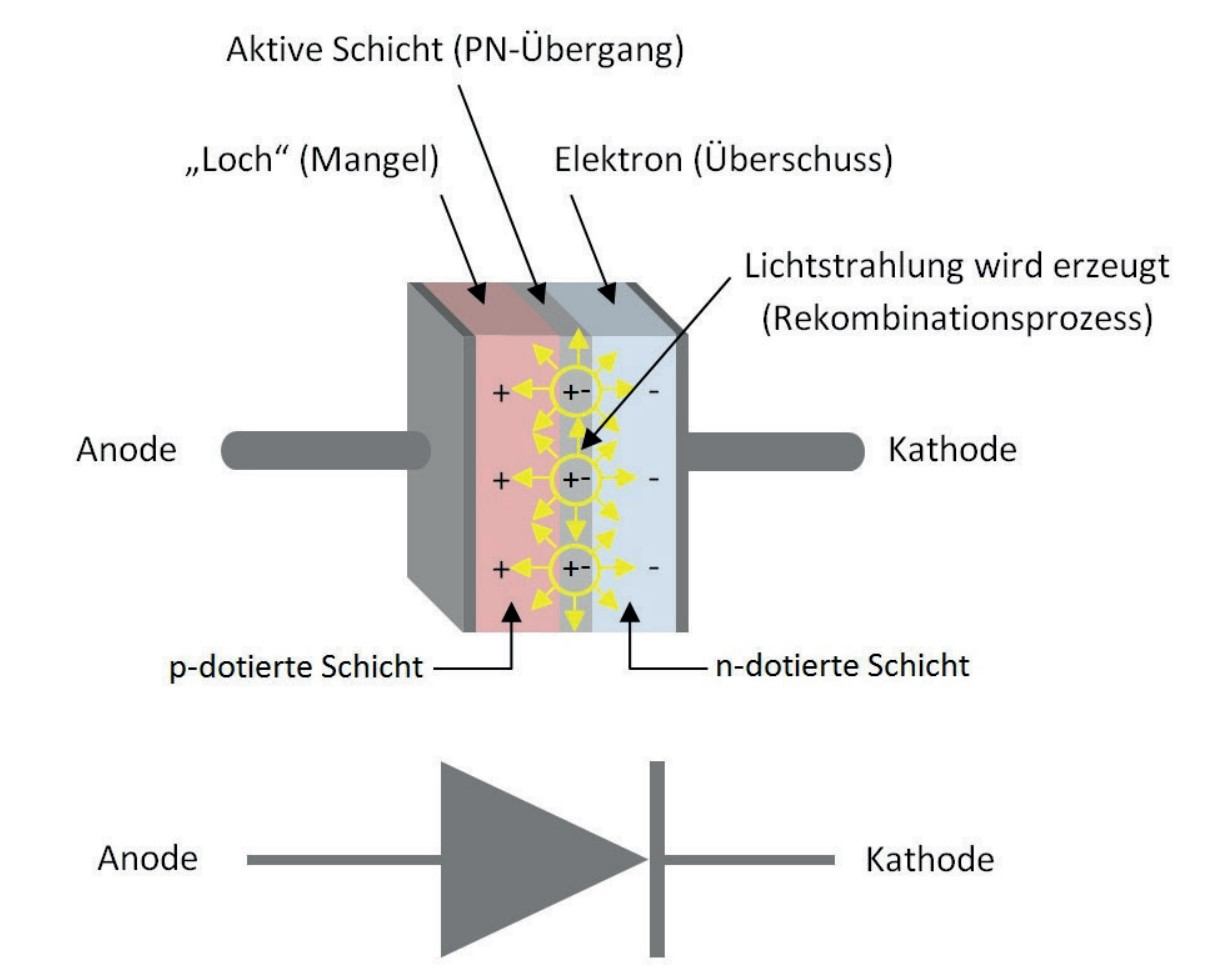
\includegraphics[width=0.65 \textwidth]{LED.jpg}
	\caption[Strahlungserzeugung in der LED am pn-Übergang]{Strahlungserzeugung in der LED am pn-Übergang} \cite{slabke}
	\label{fig:LED}
\end{figure}

Der Grundsatz der Lichterzeugung in einer \gls{acr:LED} beruht auf einem Halbleiterkristall, der durch das Einbringen vom Fremdatomen so dotiert ist, dass in der Diode zwei Gebiete entstehen. In einem Gebiet entsteht ein Elektronenüberschuss und in dem anderen Gebiet entstehen Löcher. Durch das injizieren von Elektronen aus der positiv dotierten Seite in die Sperrschicht, rekombinieren sich Löcher und Elektronen, wodurch Energie in Form von Licht abgegeben wird.\cite{slabke} Die Farbe hängt dabei vom Halbleitermaterial und der genauen Dotierung ab. Zudem ist dieser Rekombinationsprozess stark Temperaturabhängig. Dies wird in einem noch folgenden Kapitel näher erläutert.

\begin{figure}[h]
	\centering
	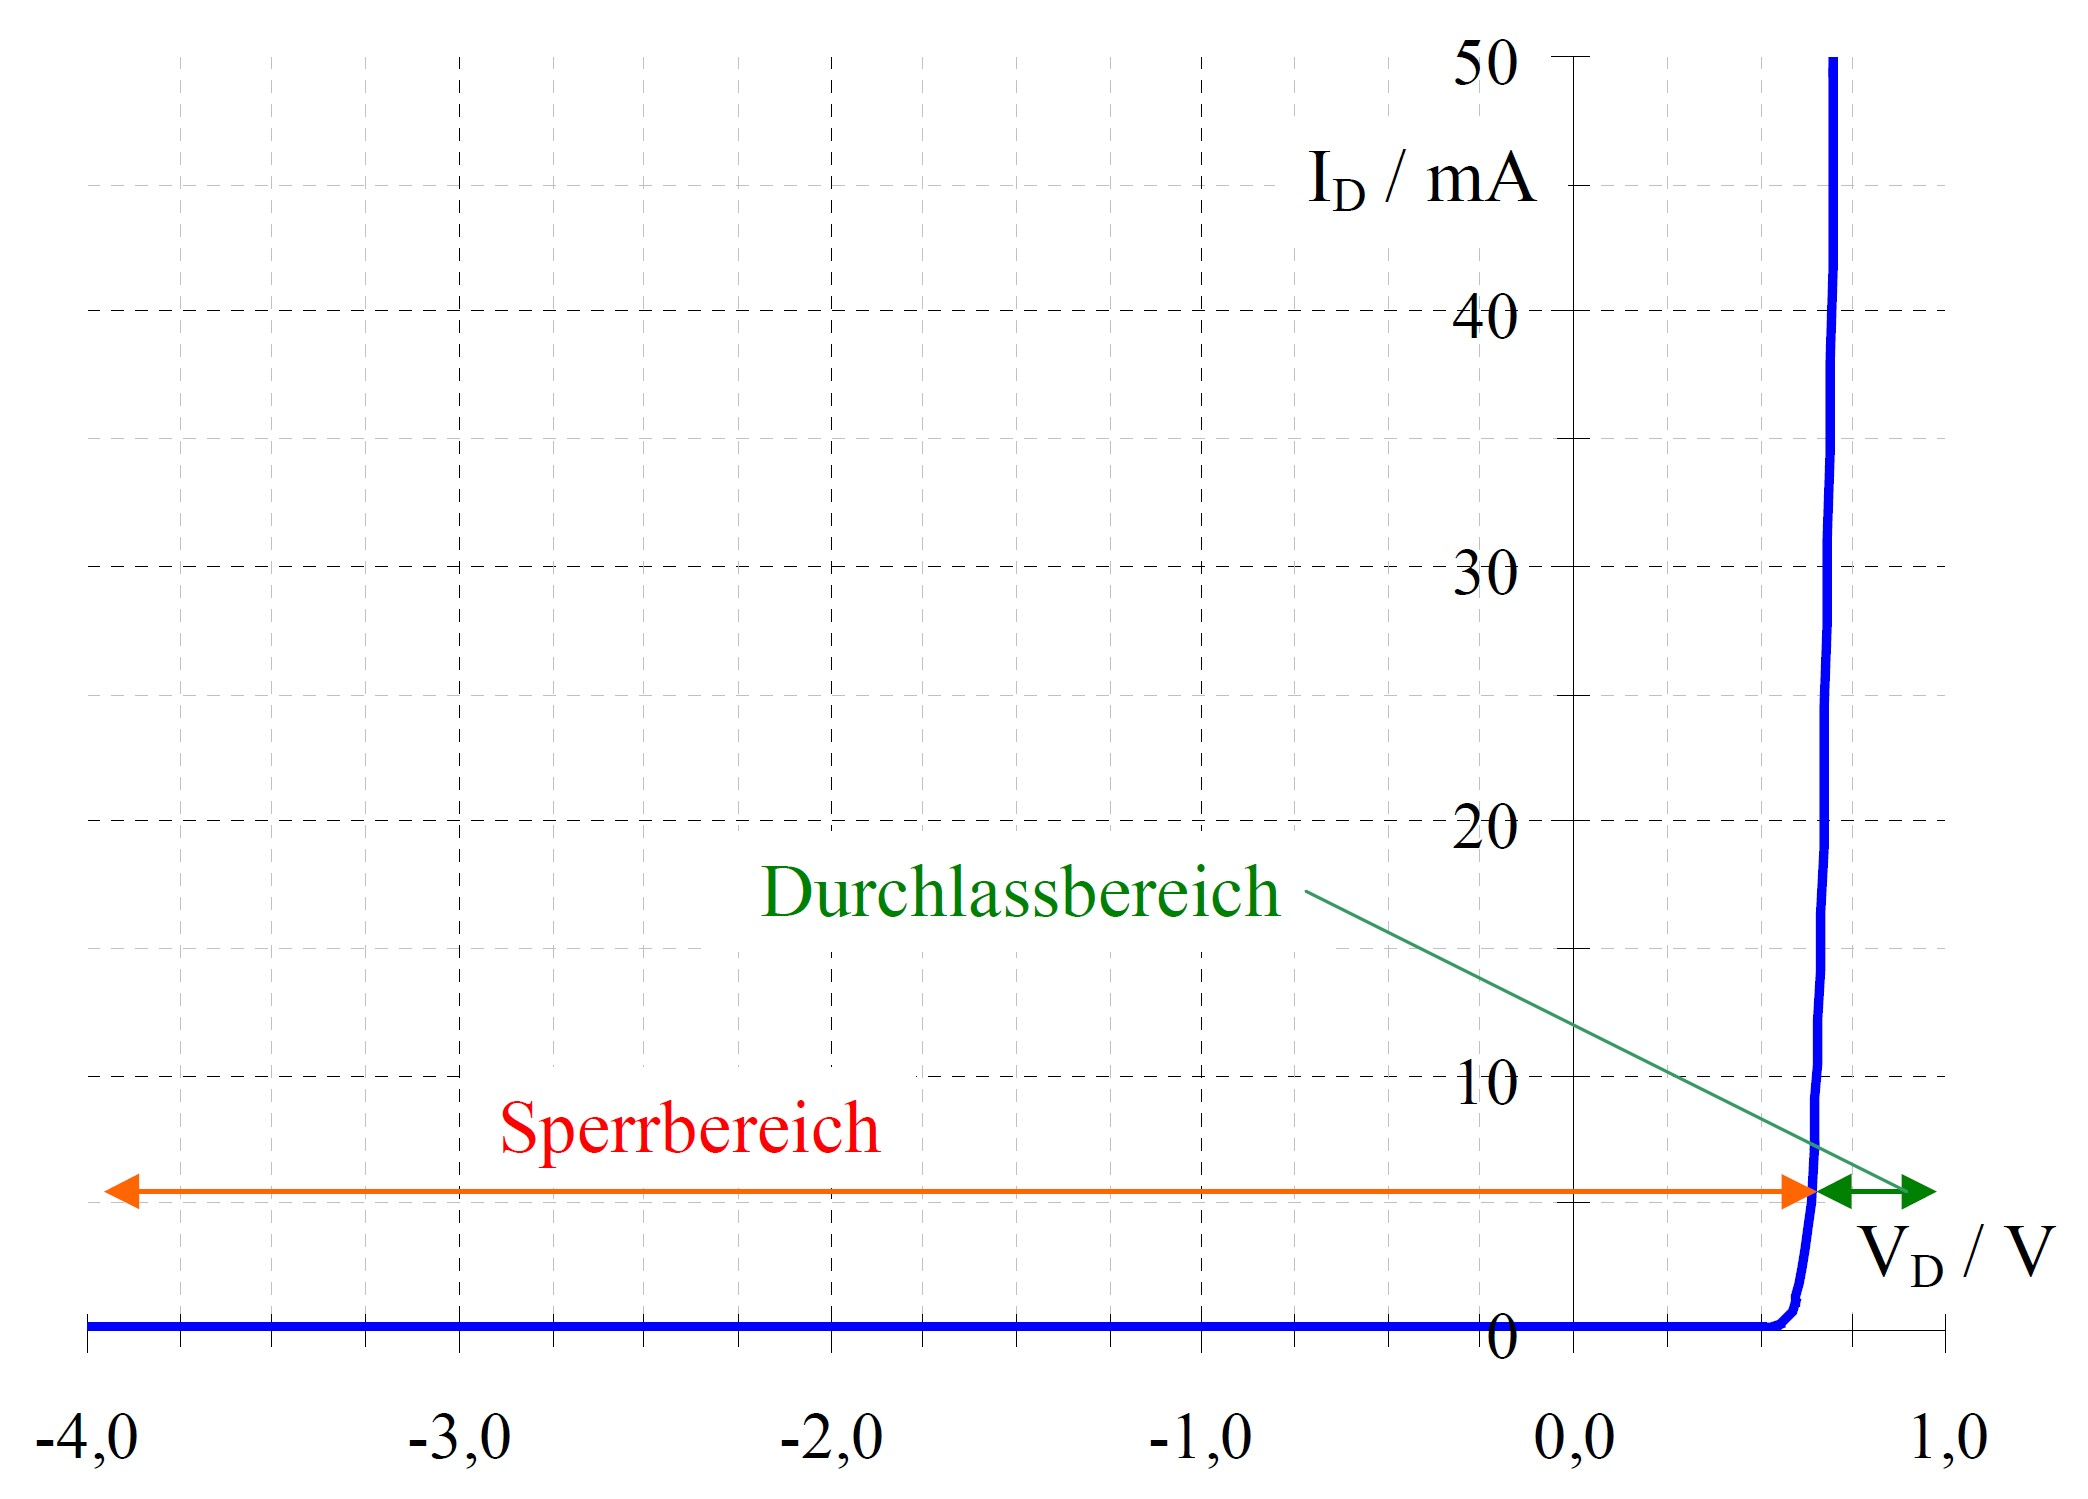
\includegraphics[width=0.65 \textwidth]{Kennlinie.jpg}
	\caption[Diodenkennlinie]{Diodenkennlinie} 
	\cite{Vorlesung_Elektonik}
	\label{fig:Kennlinie}
\end{figure}


In der Abbildung ~\ref{fig:Kennlinie} ist die Strom-/Spannungskennlinie einer Diode in Durchlassrichtung
dargestellt. Die Kennlinie einer LED hat den selben Verlauf, jedoch ist die Durchlassspannung
je nach gewählter Farbe nicht bei ca. 0.7V sondern bei bis zu 4V bei
einer blauen LED. 

\begin{figure}[h]
	\centering
	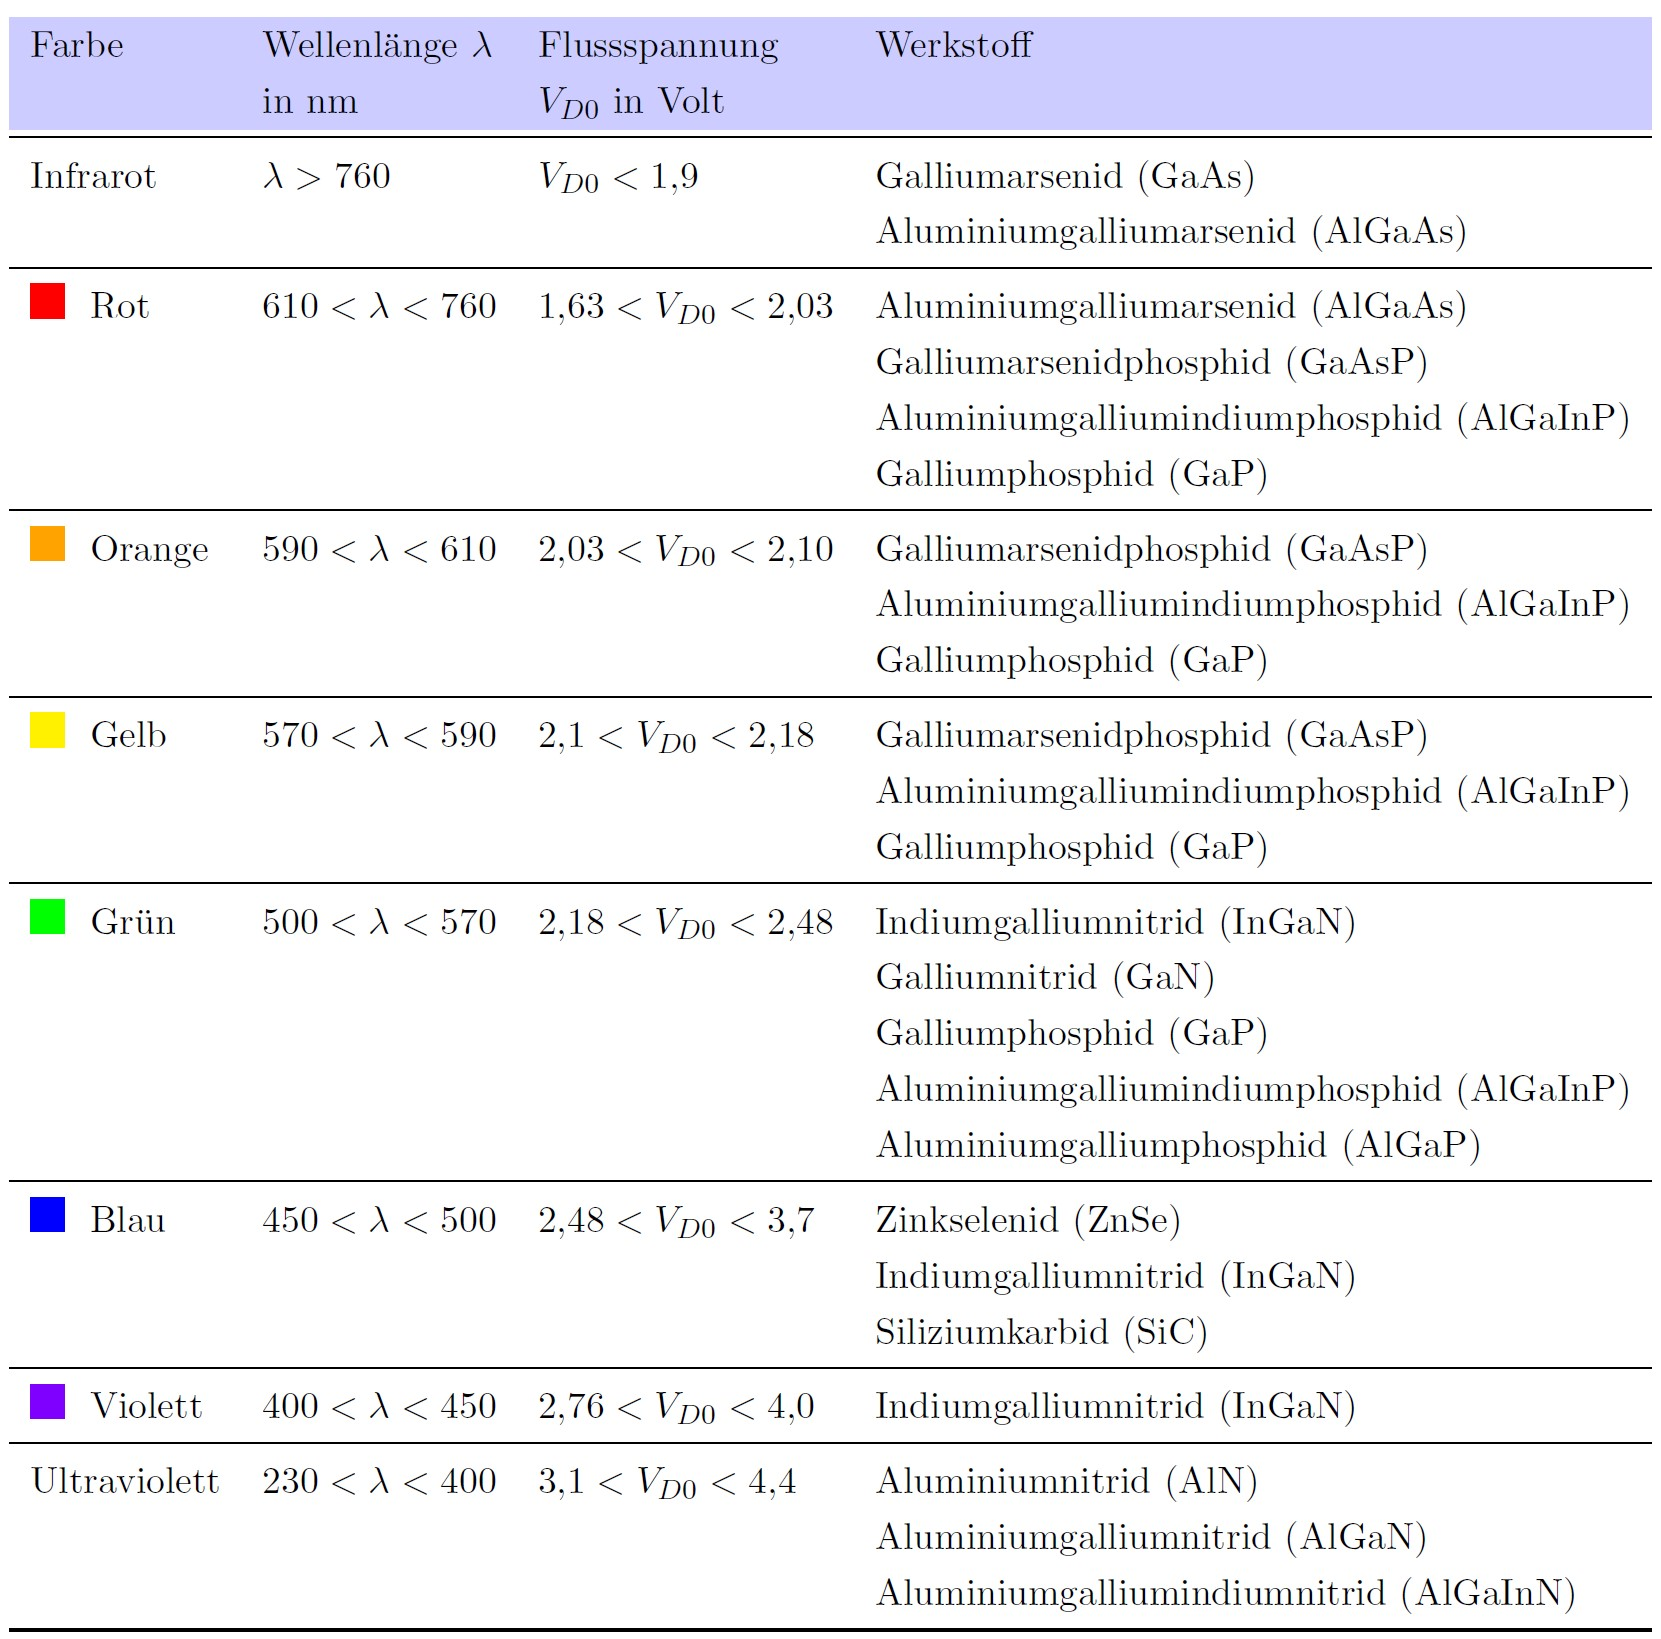
\includegraphics[width=0.85 \textwidth]{Flussspannung.jpg}
	\caption[Flussspannungen von \gls{acr:LED}s verschiedener Farben]{Flussspannungen von \gls{acr:LED}s verschiedener Farben} 
	\cite{Vorlesung_Elektonik}
	\label{fig:Flussspannung}
\end{figure}

Wie in Abbildung ~\ref{fig:Kennlinie} illustriert ist, ändert sich die Spannung in ihrem Verlauf
ab einem gewissen Punkt nur noch minimal. Das bedeutet, dass sich ab einer gewissen
angelegten Spannung lediglich der Strom noch weiter erhöhen kann. Da die
Leuchtintensität der \gls{acr:LED} von dieser Höhe des Stromdurchflusses abhängt, führt dies zu der
Betrachtung, den durchfließenden Strom statt der angelegten Spannung zu regulieren.
Stellt man nun den durch die \gls{acr:LED} fließenden Strom mit der Ausgangsleistung
ins Verhältnis, ergibt sich ein Zusammenhang wie ihn Abbildung ~\ref{fig:Helligkeit} zeigt. 

\begin{figure}[H]
	\centering
	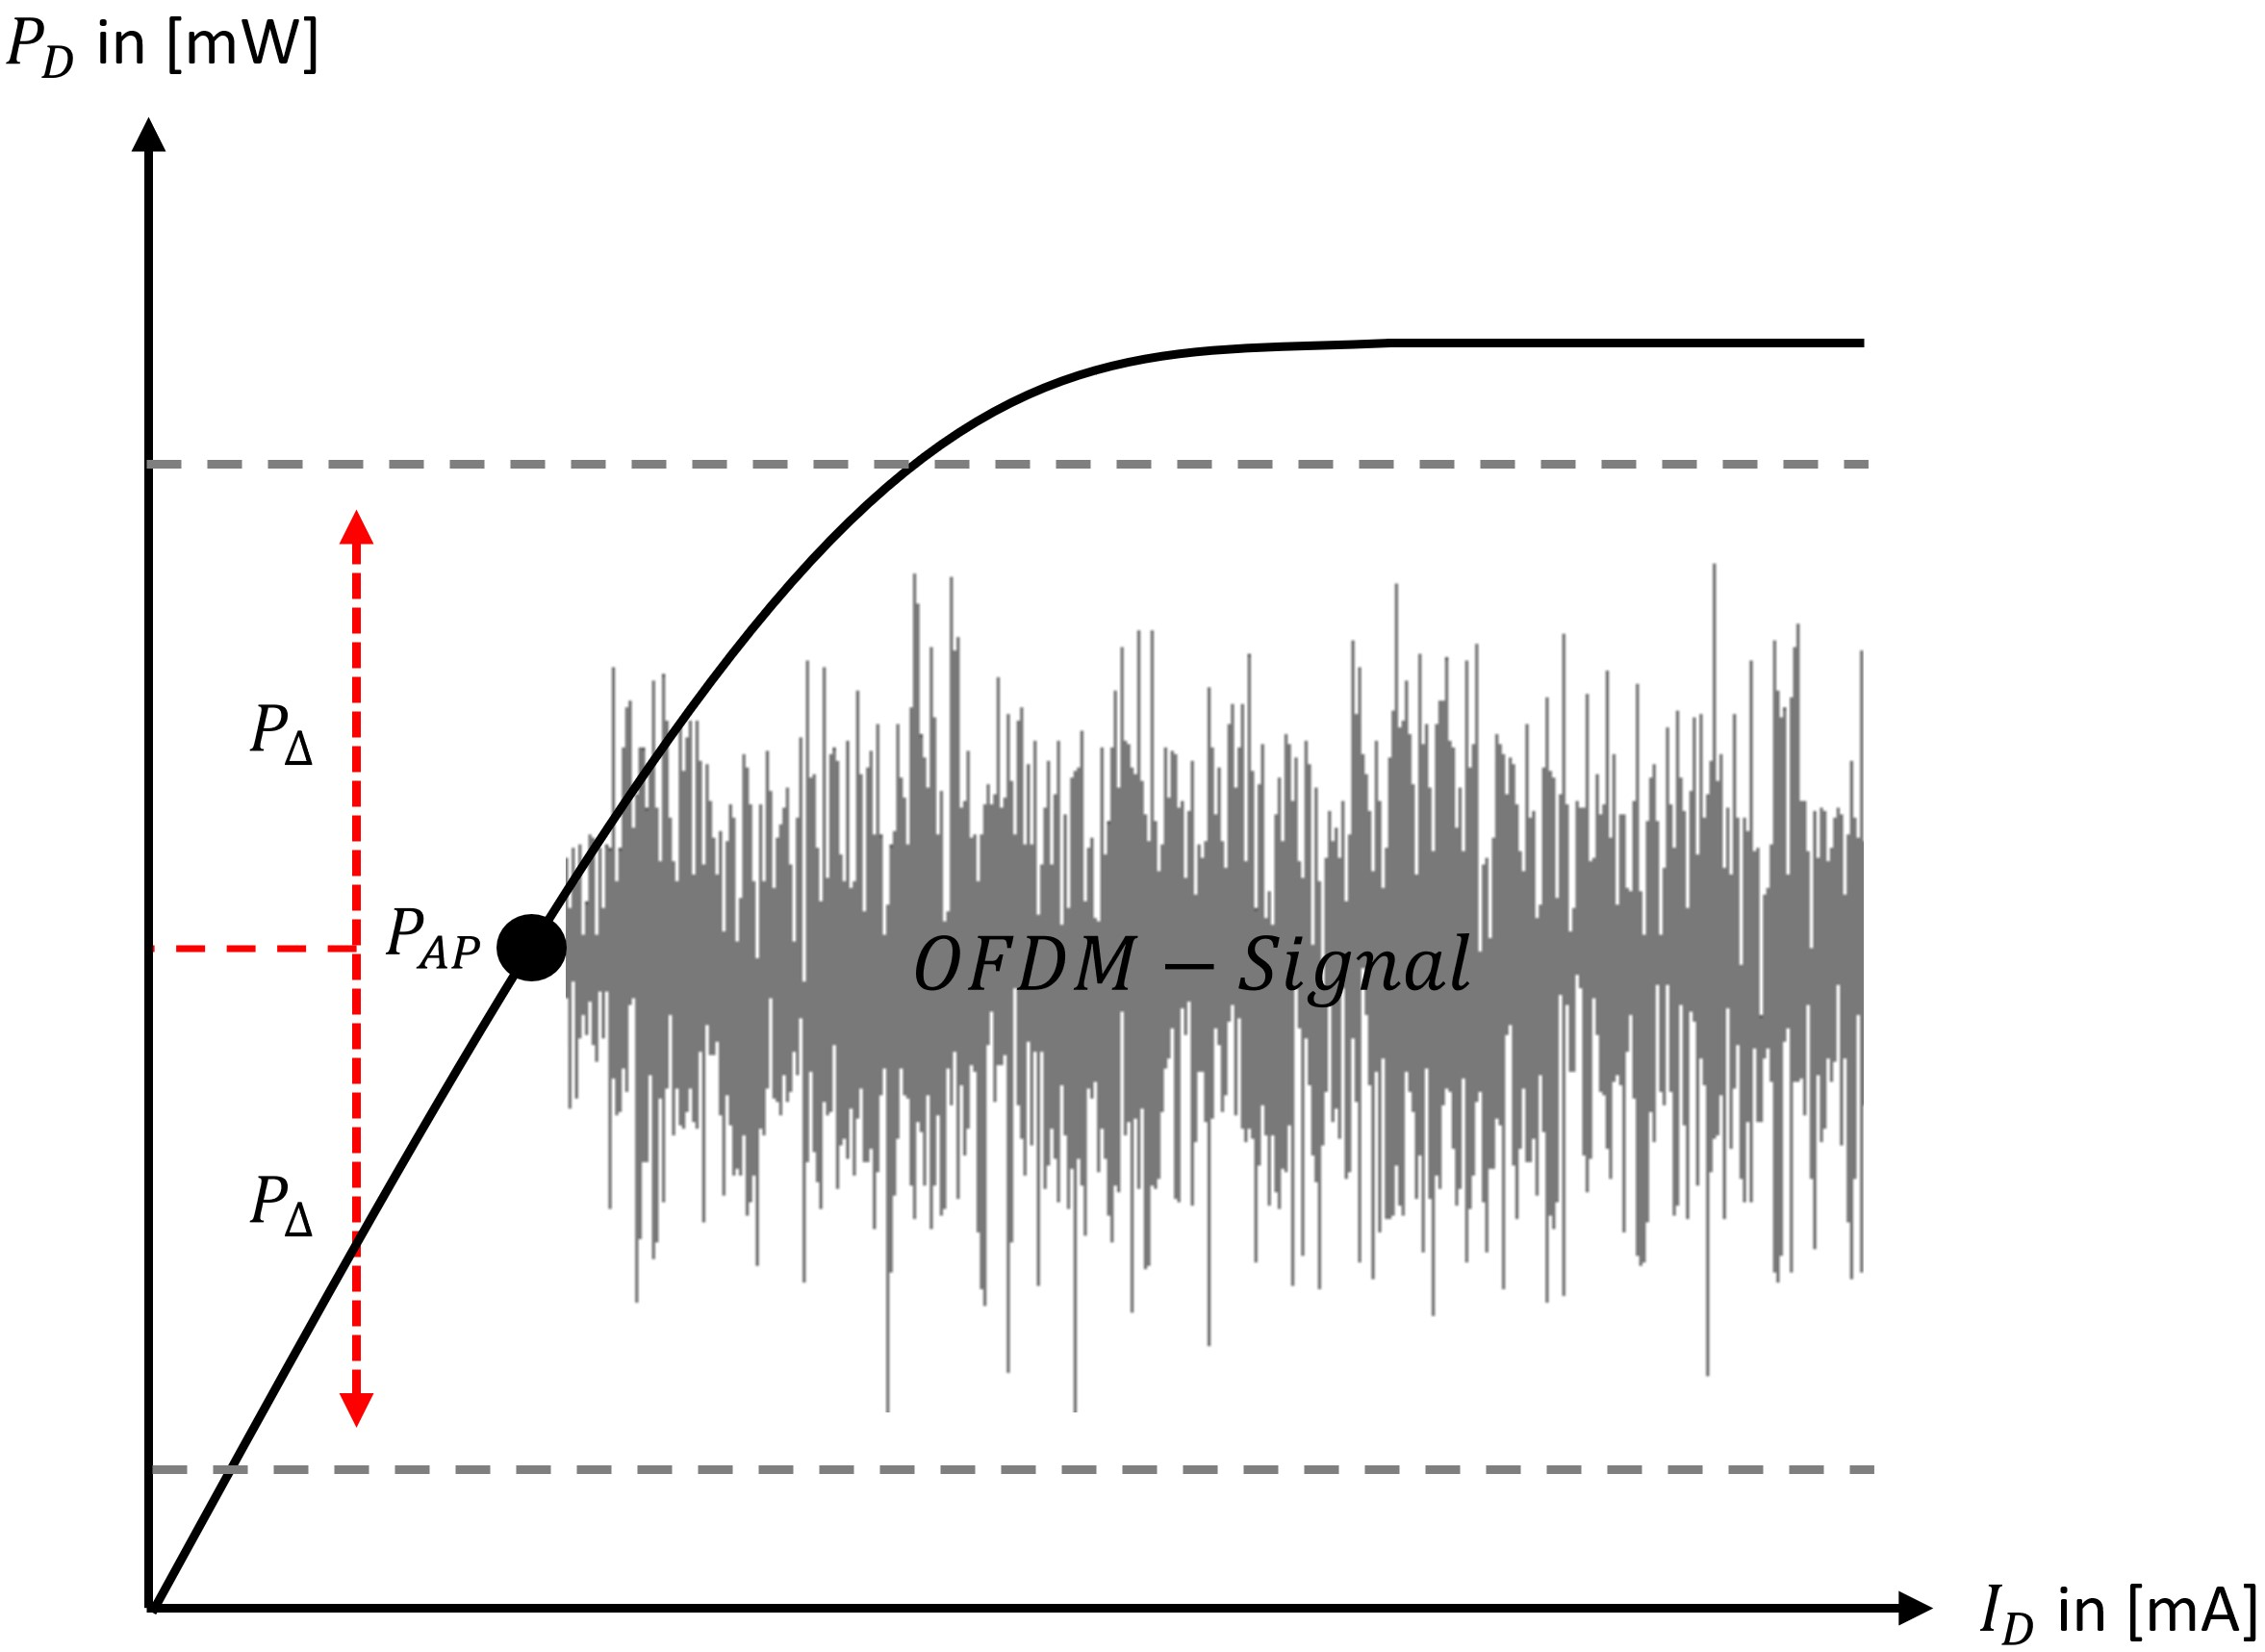
\includegraphics[width=0.78 \textwidth]{Helligkeit.jpg}
	\caption[Kennlinie einer Diode – Lichtleistung zu fließendem Strom]{Kennlinie einer Diode – Lichtleistung zu fließendem Strom} 
	\cite{Eigen}
	\label{fig:Helligkeit}
\end{figure}

An dieser Stelle wird verdeutlicht, dass es zwei außerordentlich nicht-lineare Abschnitte in der Kennlinie gibt, welche sich durch ihre stark nicht-linearen Eigenschaften keineswegs zur Datenübertragung eignen. Zwischen diesen Bereichen um die etwa mittlere Lichtleistung, gibt es jedoch einen linearen Bereich, welcher sich ausgezeichnet für die Übertragung von Daten eignet. Dies bedeutet, dass die LED auf einem festen Arbeitspunkt AP betrieben werden muss. Dieser Arbeitspunkt liefert der Diode einen immensen Aktionsradius. Wodurch eine maximale Aussteuerung der Amplitude des Signals und somit eine verbesserte Konstellation zur Signalübertragung gewährleistet wird.


\subsection{Der Operationsverstärker}
\label{subsec:Unterabschnitt12}

„Im Grunde besteht kein Unterschied zwischen einem normalen Verstärker und einem Operationsverstärker. Beide dienen dazu, Spannungen bzw. Ströme zu verstärken. Während die Eigenschaften eines normalen Verstärkers jedoch durch seinen inneren Aufbau vorgegeben sind, ist ein Operationsverstärker so beschaffen, dass seine Wirkungsweise überwiegend durch eine äußere Gegenkopplungs-Beschaltung bestimmt werden kann. Um dies zu ermöglichen, werden Operationsverstärker als gleichspannungsgekoppelte Verstärker mit hoher Verstärkung ausgeführt. Damit keine zusätzlichen Maßnahmen zur Arbeitspunkteinstellung erforderlich werden, verlangt man ein Eingangs- und Ausgangsruhepotential von 0V. Deshalb sind in der Regel zwei Betriebsspannungsquellen erforderlich: eine positive und eine negative.“(\cite{tietzeElectronicCircuits2008},S.491)

Ein \gls{acr:OP} kann also mit einem Differenzverstärker mit einer theoretisch unendlichen Verstärkung verglichen werden. Diese bezeichnet man als Leerlaufverstärkung. Schließlich führt das dazu, dass eine Gesamtverstärkung der Schaltung von einer zusätzlichen externen Verdrahtung abhängt. Diese wird von einem rückgekoppelten Netzwerk hergestellt und nennt sich Schleifenverstärkung.\cite{lutzHalbleiterLeistungsbauelemente2012}

\begin{figure}[H]
	\centering
	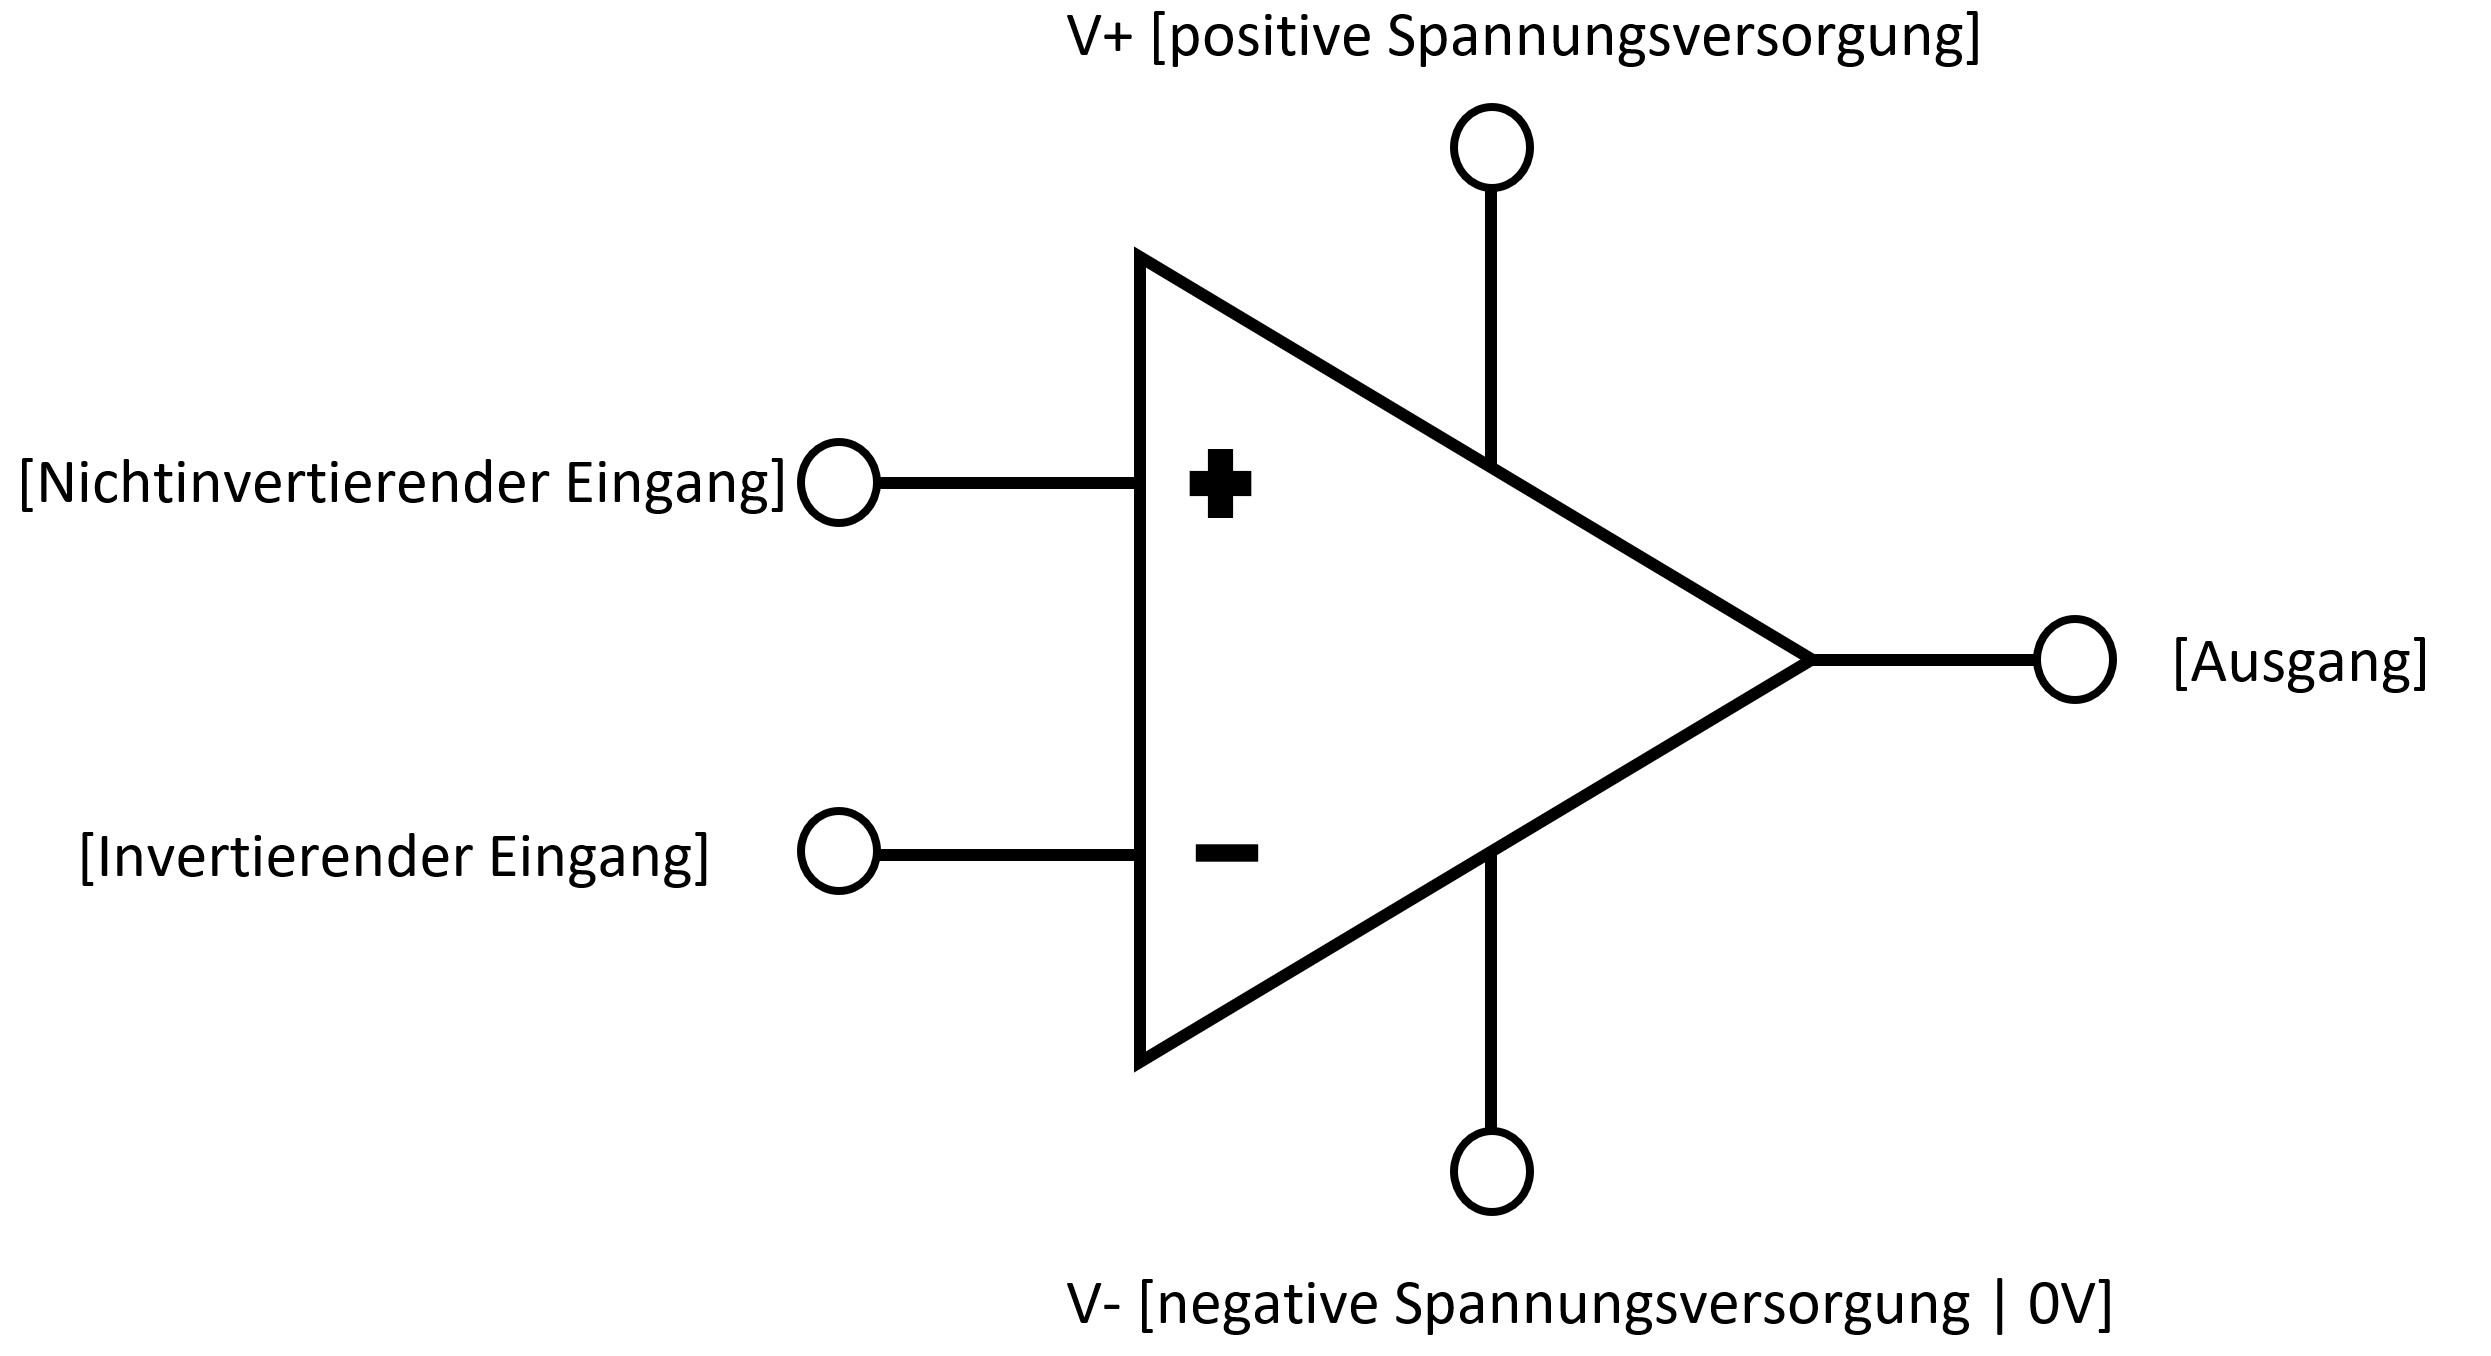
\includegraphics[width=0.7 \textwidth]{OPV.jpg}
	\caption[Operationsverstärker Anschlussschema]{Operationsverstärker Anschlussschema} 
	\gls{online:Eigen}
	\label{fig:OPV}
\end{figure}

Sie werden im Allgemeinen in Form einer integrierten Schaltung (\gls{acr:IC}) hergestellt, da die in dem Datenblatt eines Operationsverstärkers angegebenen Werte ausreichend beschrieben werden. Zudem verfügt der \gls{acr:OP} über einen invertierenden (-) und nicht-invertierenden (+) Eingang. Daraus können zwei der \gls{acr:OP}-Grundschaltungen extrahiert werden. Um das Verhältnis zwischen der Ausgangsspannung $U_{a}$ und der Eingangsspannung $U_{e}$ zu berechnen werden häufig die Parameter A und G verwendet. [Halbleiter Buch]

\begin{equation}
	\label{equ:bsp1}
	A = \frac{U_{a}}{U_{e}}
\end{equation}

Außerdem haben \gls{acr:OP}s einen unendlich großen Eingangswiderstand und einen sehr geringen Ausgangswiderstand.
Das Ruhepotential zwischen dem invertierenden und nicht-invertierenden Eingang ist beinahe Null weshalb zwischen beiden Eingängen keine Spannung abfällt. Zudem fließt kein Steuerstrom, d.h. es fließt kein Strom in die Eingänge des \gls{acr:OP}, da diese einen unendlichen Eingangswiderstand besitzen.\cite{federauOperationsverstaerker2017}
\begin{figure}[H]
	\centering
	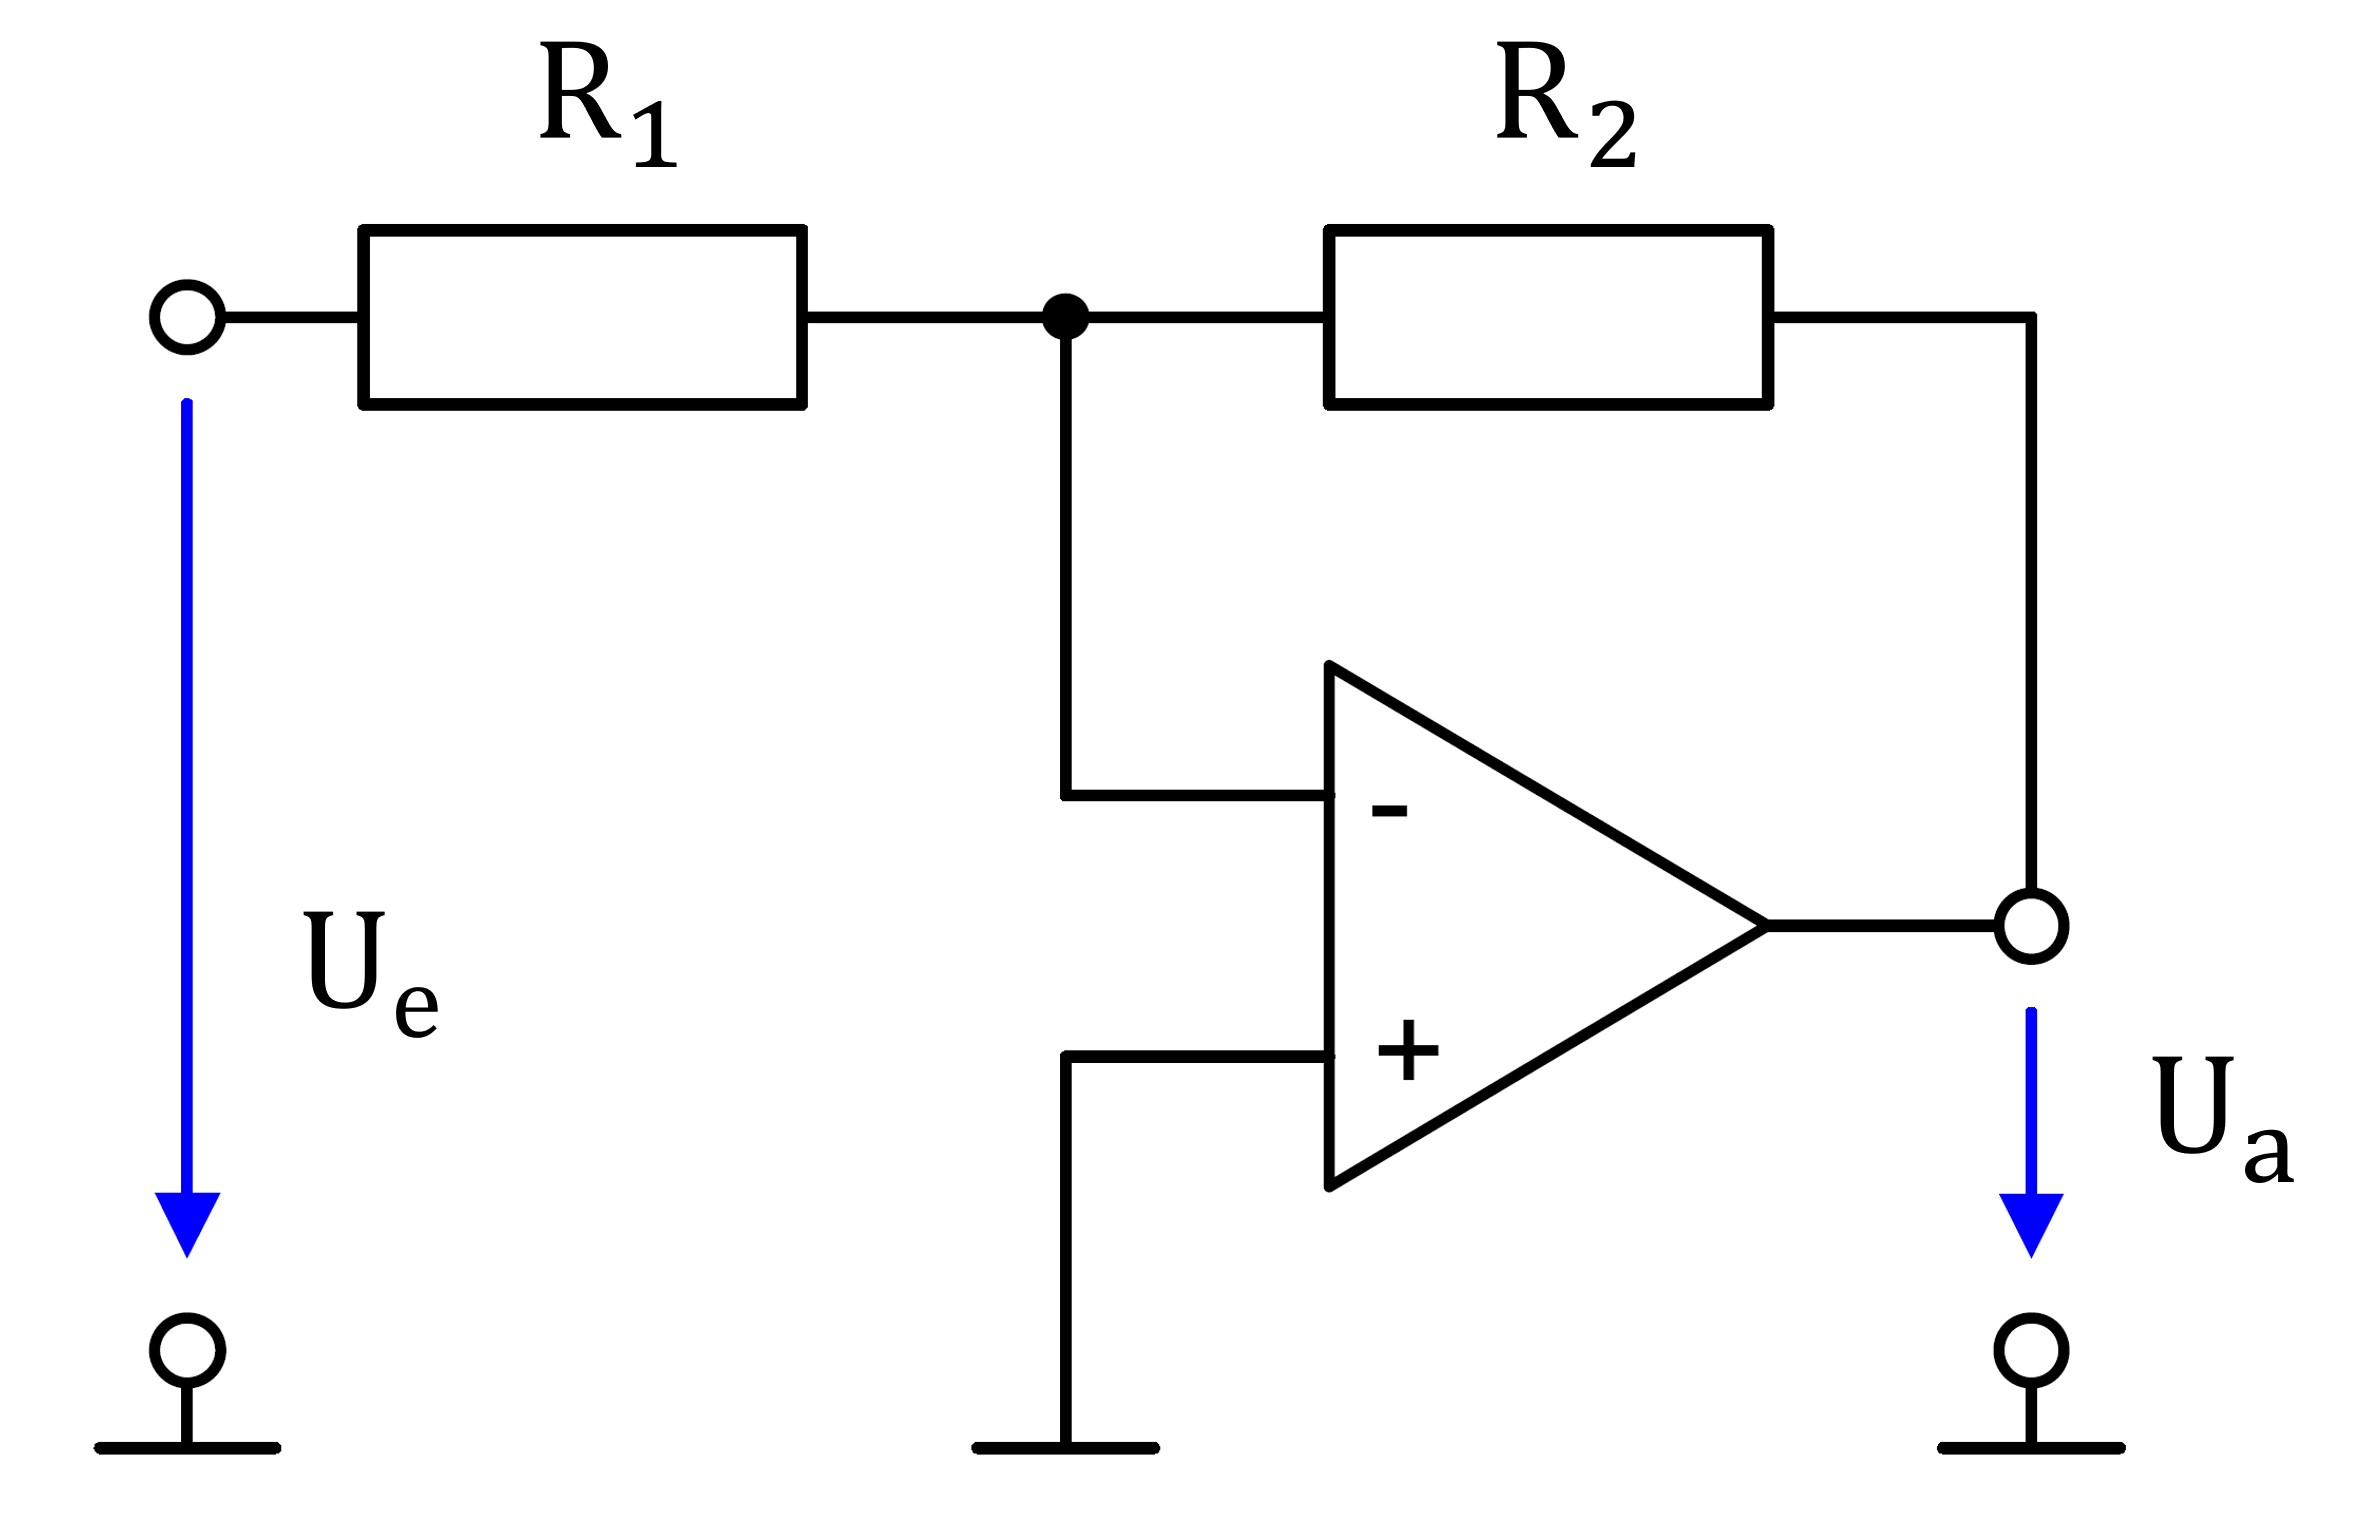
\includegraphics[width=0.7 \textwidth]{invOP.jpg}
	\caption[Invertierender Operationsverstärker]{Invertierender Operationsverstärker} 
	\gls{online:Eigen}
	\label{fig:ninvOP}
\end{figure}

Abbildung ~\ref{fig:ninvOP} zeigt die klassische Schaltung eines invertierenden Operationsverstärkers mit
Rückkopplungszweig. Dieser definiert über den Widerstand $R_{2}$ die Schleifenverstärkung, indem auf den invertierten Eingang ein Teil des Ausgangssignals zurückgeführt wird.  Bei einem steigenden Ausgangssignal wird so dem steigenden Eingangssignal entgegengewirkt. Dies gewährleistet, dass das Ausgangssignal nicht unendlich verstärkt werden kann. Der invertierende Eingang wird mit Masse verbunden. Zuletzt wird hier die Spannungsverstärkung $A$ der invertierenden Grundschaltung über den Rückkopplungspfad bestimmt. Diese ergibt sich hier also zu: 

\begin{equation}
	\label{equ:bsp1}
	A = - \frac{R_{2}}{R_{1}}
\end{equation}

und das negative Vorzeichen bedeutet, dass hier eine Phasendrehung des Signals um 180$\circ$ stattgefunden hat.Der invertierende Verstärker besitzt zudem die Fähigkeit Signale zu dämpfen. Daher wird er häufig für Filterschaltungen und messtechnische Zwecke benutzt. 

Die folgende Abbildung ~\ref{fig:ninvOP} illustriert den nichtinvertierenden Operationsverstärker in seiner Grundschaltung. Die Spannungsverstärkung berechnet sich anhand der Spannungsteiler Beziehung

\begin{equation}
	\label{equ:bsp1}
	U_{a} = U_{e} \cdot \frac{R_{1} + R_{2}}{R_{1}} = U_{e} \cdot (1+ \frac{R_{2}}{R_{1}})
\end{equation}
daraus ergibt sich dann
\begin{equation}
	\label{equ:bsp1}
	A = \frac{U_{a}}{U_{e}} = 1+ \frac{R_{2}}{R_{1}}
\end{equation}
Wegen seines kleinen Ausgangs- und großen Eingangswiderstandes eignet sich diese \gls{acr:OP}-Schaltung sehr gut als  Wechselspannungsverstärker und Impedanzwandler. Die Übertagungskennlinie ist in Abbildung ~\ref{fig:aussteuer} dargestellt. 

\begin{figure}[H]
	\centering
	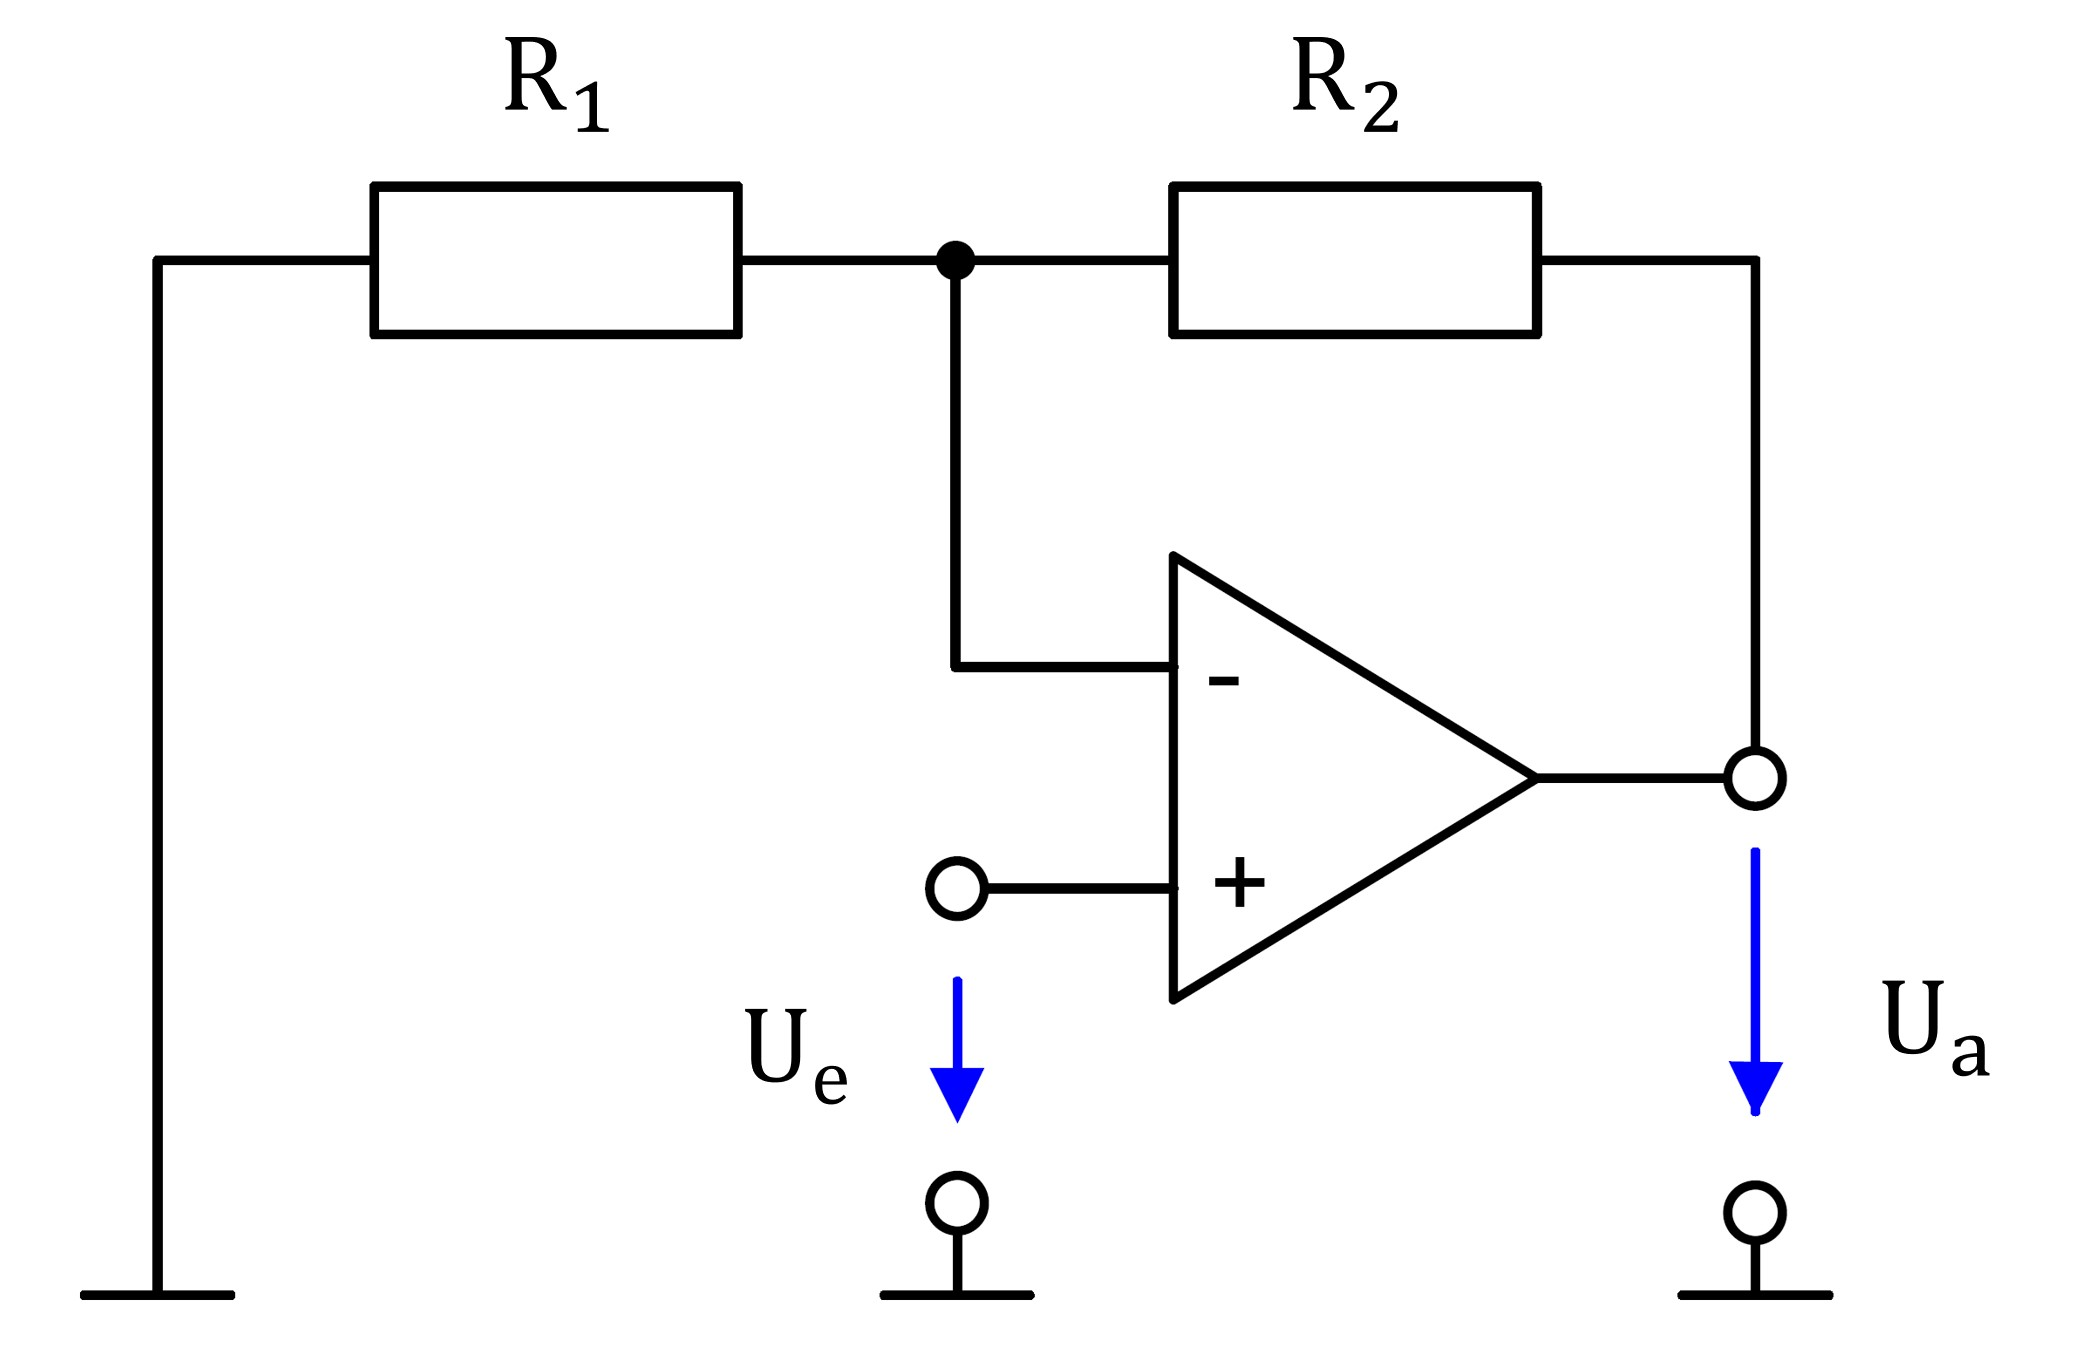
\includegraphics[width=0.7 \textwidth]{ninvOP.jpg}
	\caption[Nichtinvertierender Operationsverstärker]{Nichtinvertierender Operationsverstärker} 
	\gls{online:Eigen}
	\label{fig:invOP}
\end{figure}

Es zeigt auch die maximale Aussteuerbarkeit am Ausgang der \gls{acr:OP}s, welche innerhalb $V-$ < $U_{a}$ < $V+$ liegt. Werden entweder positive oder negative Grenze erreicht, kann $U_{a}$ nicht weiter ansteigen. Dieser Zustand nennt sich Übersteuerung. Die klassischen Aussteuergrenzen liegen in etwa 1V unter der Versorgungsspannung.\cite{federauOperationsverstaerker2017}

\begin{figure}[H]
	\centering
	\includegraphics[width=0.85 \textwidth]{aussteuer.jpg}
	\caption[Operationsverstärker]{Operationsverstärker} 
	\gls{online:Eigen}
	\label{fig:aussteuer}
\end{figure} 

\newpage
\subsection{Der Feldeffekttransistor}
\label{subsec:Unterabschnitt12}
Die am häufigsten eingesetzten Leistungsschutzschalter im Spannungsbereich von bis etwa 250V sind \gls{acr:MOSFET}.\gls{online:mosfet}


Sie sind eine Sonderform der Transistoren welche auch unipolare Transistoren genannt werden. Sie besitzen einen Kanal aus Halbleitermaterial, auf dem Horizontal zur Stromrichtung ein elektrisches Feld entsteht, welches den Querschnitt des Kanals verändert. Damit wird der Stromfluss durch das Bauteil geregelt. Im Field-Effect Transistor (FET) steuert eine Spannung den Strom. Es gibt vier Grundbauformen von \gls{acr:MOSFET}. Einen \gls{acr:NMOS} und einen \gls{acr:PMOS} Typus und davon jeweils eine selbstsperrende und einen selbstleitende Variante. Im Anwendungsfall dieser Thesis wird ein \gls{acr:NMOS} verwendet. \cite{heringElektrotechnikUndElektronik2018}

\newpage
\subsection{Das Digital Potentiometer}
\label{subsec:Unterabschnitt12}

Um den Strom durch die \gls{acr:LED} digital zu regulieren und demgemäß für die Datenübertragung die Helligkeit der \gls{acr:LED} zu variieren, wird ein Digitalpotentiometer benötigt. Hierfür wurde der \gls{acr:IC} MCP42010 in der 10k$\ohm$–Variante mit 2 Kanälen ausgewählt. Dieses Digitalpotentiometer kann über ein \gls{acr:SPI} mittels eines Arduino angesteuert werden um dessen Widerstandswert in 256 Schritten zu verändern. Dies ermöglicht eine Variation des Widerstandes in einem Bereich zwischen 52$\ohm$ (00h) und 10k$\ohm$ (FFh) in 39$\ohm$ Schritten. 
Die vom \gls{acr:IC} vorgeschriebene Versorgungsspannung von 5V stellt der Spannungsversorgungspin des Arduino bereit. Außerdem kann dem Datenblatt des \gls{acr:IC}s die Information entnommen werden, dass dessen Eingangsspannungsbereich an den Widerstandseingängen maximal zwischen -0.5V und 6V liegen darf. Da der IC in dieser Schaltung mit 5V betrieben wird, dürfen die Widerstandseingänge mit einer Spannung von maximal -0.6V bis 6V belastet werden. Das ist ein äußerst wichtiges Kriterium für die Auslegung er Schaltung, da hier über die Grenzen der maximalen Amplitude entschieden werden muss, um vor unerwünschten Nebeneffekten vorzubeugen.

\begin{figure}[H]
	\centering
	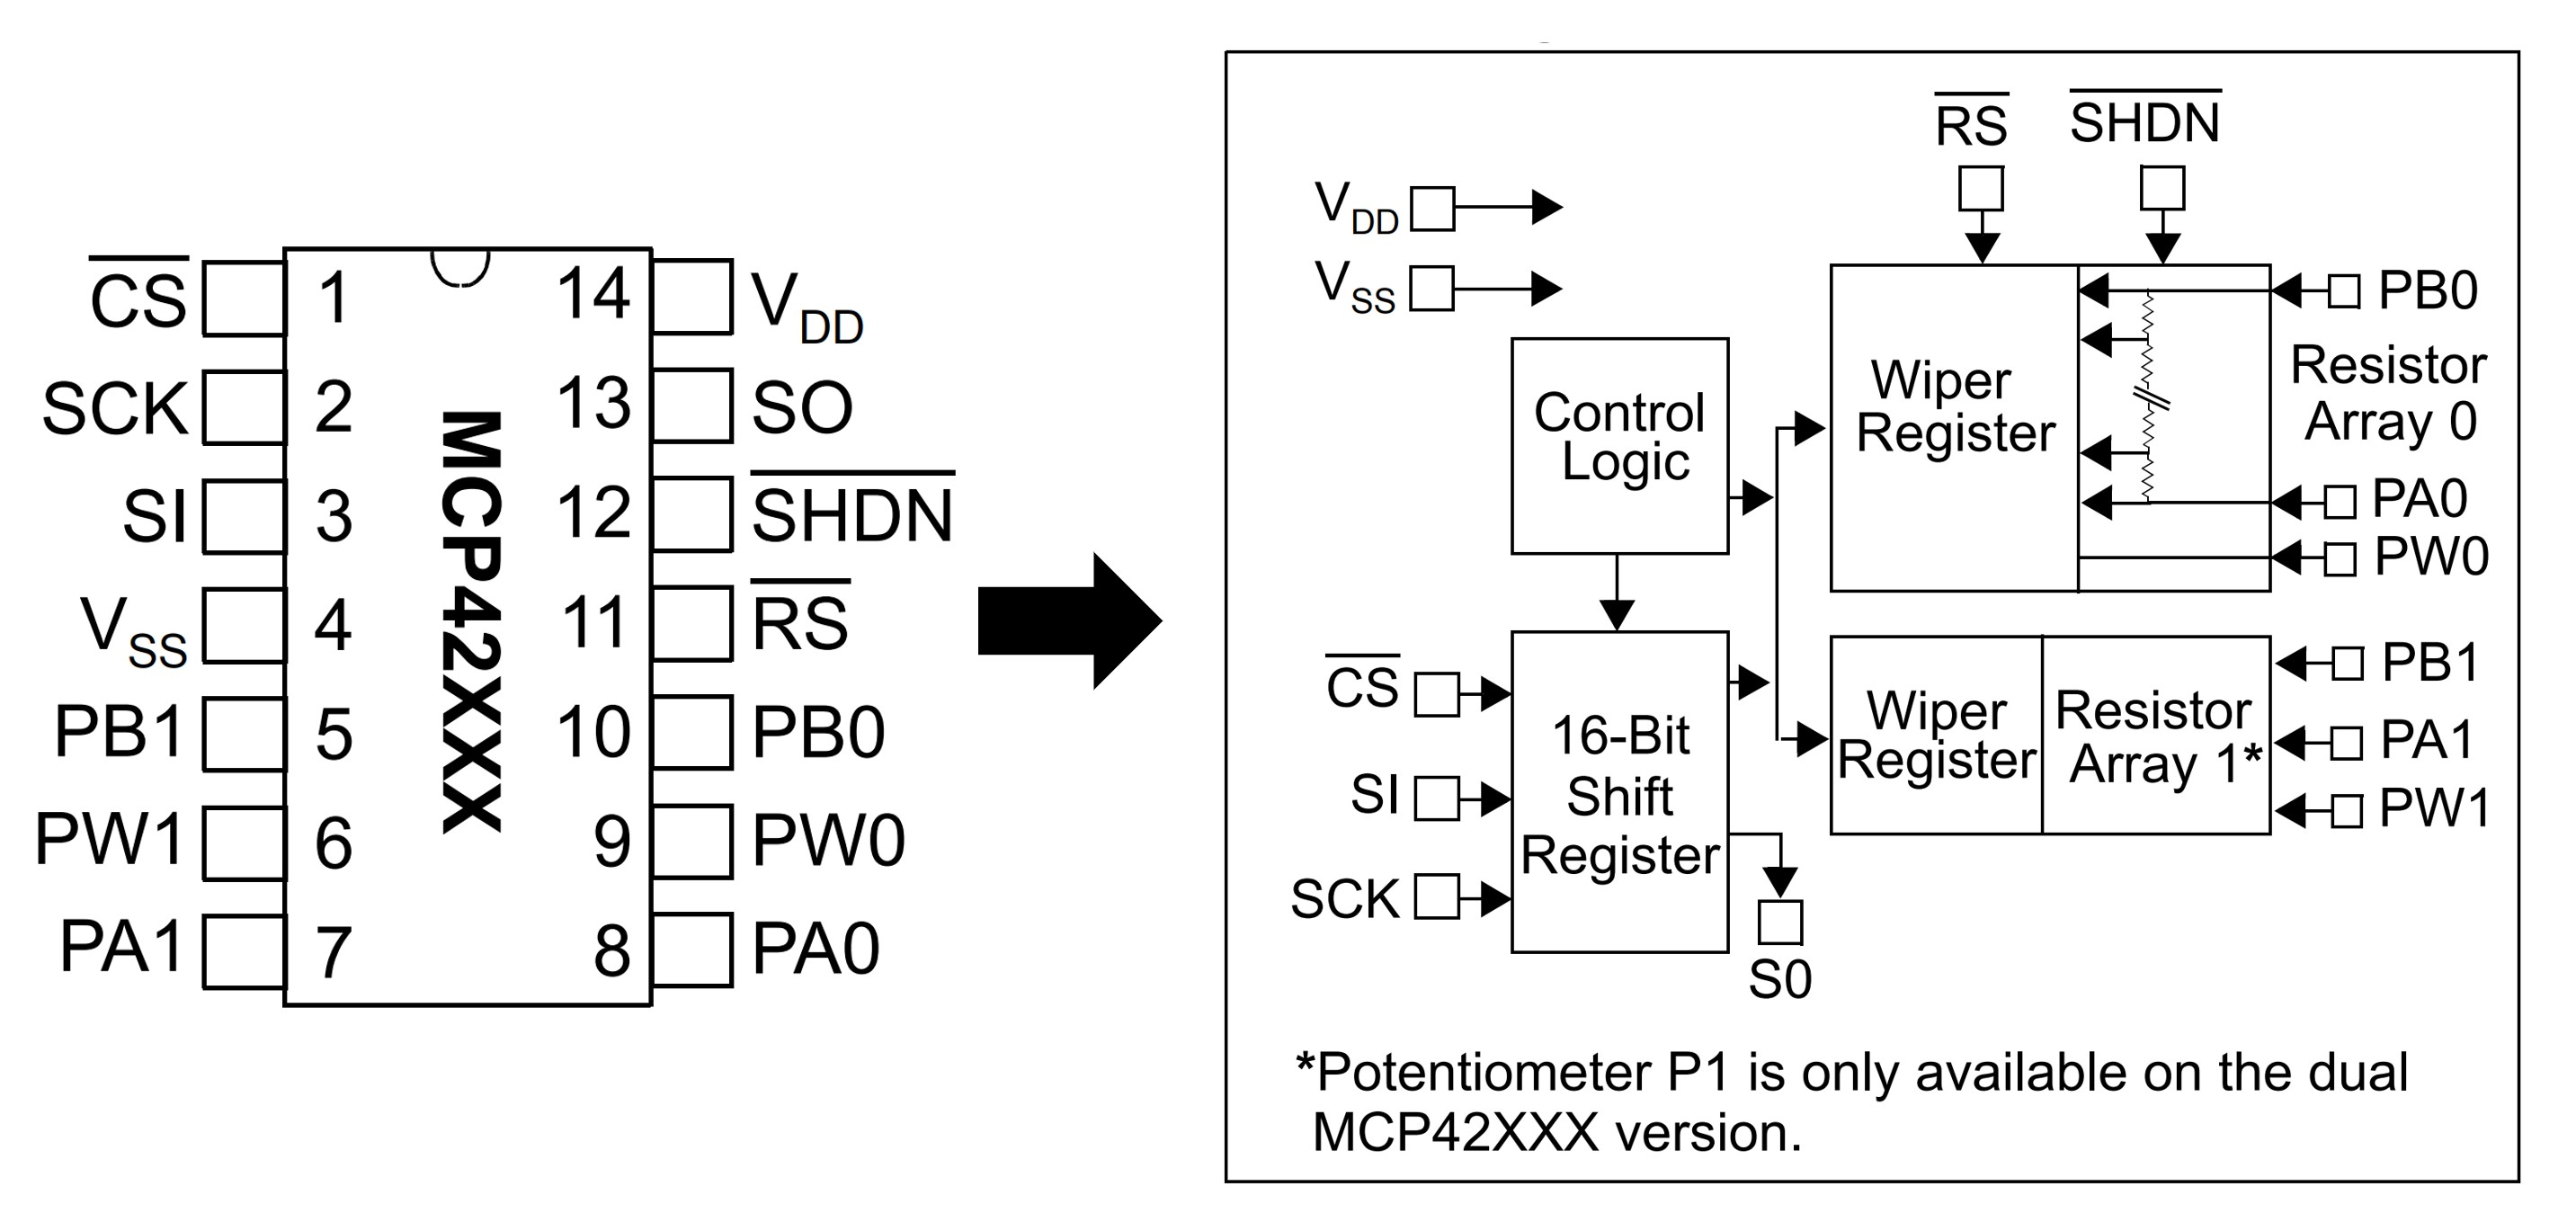
\includegraphics[width=0.8 \textwidth]{MCP.jpg}
	\caption[Aufbau des MCP42010]{Aufbau des MCP42010} 
	\cite{MCP42}
	\label{fig:MCP}
\end{figure}

Die Funktion der einzelnen Pins und wie man den \gls{acr:IC} mit dem Arduino verbindet wird in nachfolgender Tabelle~\ref{tab:pinmcp} beschrieben. 
\begin{table}[htb]
	\begin{center}
		\begin{tabular}[H]{cccc}	
			\toprule
			\textbf{Pin Nr.} & \textbf{Name}  &\textbf{Funktion} & \textbf{Arduino Pin Nr.} \\
			\midrule
			1 & $\overline{CS}$ & Chip Select &  10 \\
			2 & SCK & Serial Clock &  13 \\
			3 & SI & Serial Data Input&  11 \\
			4 & $V_{SS}$ & Ground &  Ground \\
			5 & PB1 & Terminal B Connection For Pot 1 & X \\
			6 & PW1 & Wiper Connection For Pot 1 &  OP-1 Minus \\
			7 & PA1& Terminal A Connection For Pot 1 &  OP-1 Out  \\
			8 & PA0& Terminal A Connection For Pot 0 &  5V \\
			9 & PW0& Wiper Connection For Pot 0 & OP-2 Offset \\
			10 & PB0 & Terminal B Connection For Pot 0 &  Ground \\
			11 & $\overline{RS}$ & Reset Input & X  \\
			12 & $\overline{SHDN}$ & Shutdown Input &X\\
			13 & SO & Data Out for Daisy-Chaining & X \\
			14 & $V_{DD}$ & Power & 5V \\
			\bottomrule
		\end{tabular}
		\caption{Anschlussinformation und Pinbelegung des MCP42010}
		\label{tab:pinmcp}
	\end{center}
\end{table}
Aufgrund des Anwendungsfalles in dieser Thesis, werden Pin 11 und Pin 12 des MCP42010 nicht benötigt und aus diesem Grund nicht am Arduino angeschlossen. 

\subsection{Der DC/DC Spannungswandler}
\label{subsec:Unterabschnitt12}

Ein Gleichspannungswandler oder auch DC-DC-Wandler, wandelt eine der Schaltung zugeführte Eingangsgleichspannung in eine geregelte Ausgangsgleichspannung, welche ein anderes Spannungsniveau als die Eingangsspannung aufweist. Diese kann beispielsweise niedriger, höher oder auch Invertiert sein.
Da die zu übertragenden Daten am Ausgang der Soundkarte als reine Wechselspannung anliegen, wird eine negative Spannungsquelle für die vorhandenen Operationsverstärker benötigt, um kein Risiko auf Datenverluste einzugehen.
Gleichspannungswandler werden grundsätzlich immer dort eingesetzt, wo die zu Verfügung stehende Eingangsspannung nicht zur Versorgung der im Schaltkreis folgenden elektronischen Bauteile passt.[AbcderPowerModuleGrundlagen.pdf] Aufgrund der Unkonventionalität sowohl eine negative als auch eine positive Spannungsquelle simultan an die Platine anzuschließen, wandelt der DC/DC-Spannungswandler diese negative Spannung direkt auf der Platine um. Der LT1054 wird auch ”negative voltage generator” genannt. Das ist ein Bauteil welches eine negative Ausgangsspannung erzeugt. Diese ist proportional zur Eingangsspannung $V_{CC}$. Zum nutzen dieses Bauteiles als einfachen DC-DC-Wandler mit invertierender funktion muss es laut Datenblatt an den Ausgängen mit zusätzlichen Kondensatoren beschalten werden. Aufgrund dessen, dass der DC-DC-Wandler mit negativen Spannungen arbeitet, ist es signifikant auf die Polung der Kondensatoren zu achten, im Falle der Nutzung von Elektrolytkondensatoren. Jene sind unidirektional. Dies ist in Abbildung~\ref{fig:DCDC} illustriert. Zusätzlich ist zu erkennen, dass am negativen Ausgang des DC-DC-Wandlers nicht genau -12V anliegen sondern etwa -11.35V. Dies ist auf den Wirkungsgrad des DC-DC-Wandlers zurückzuführen und ist unter - Voltage Loss - im Datenblatt zu finden. 

\begin{figure}[H]
	\centering
	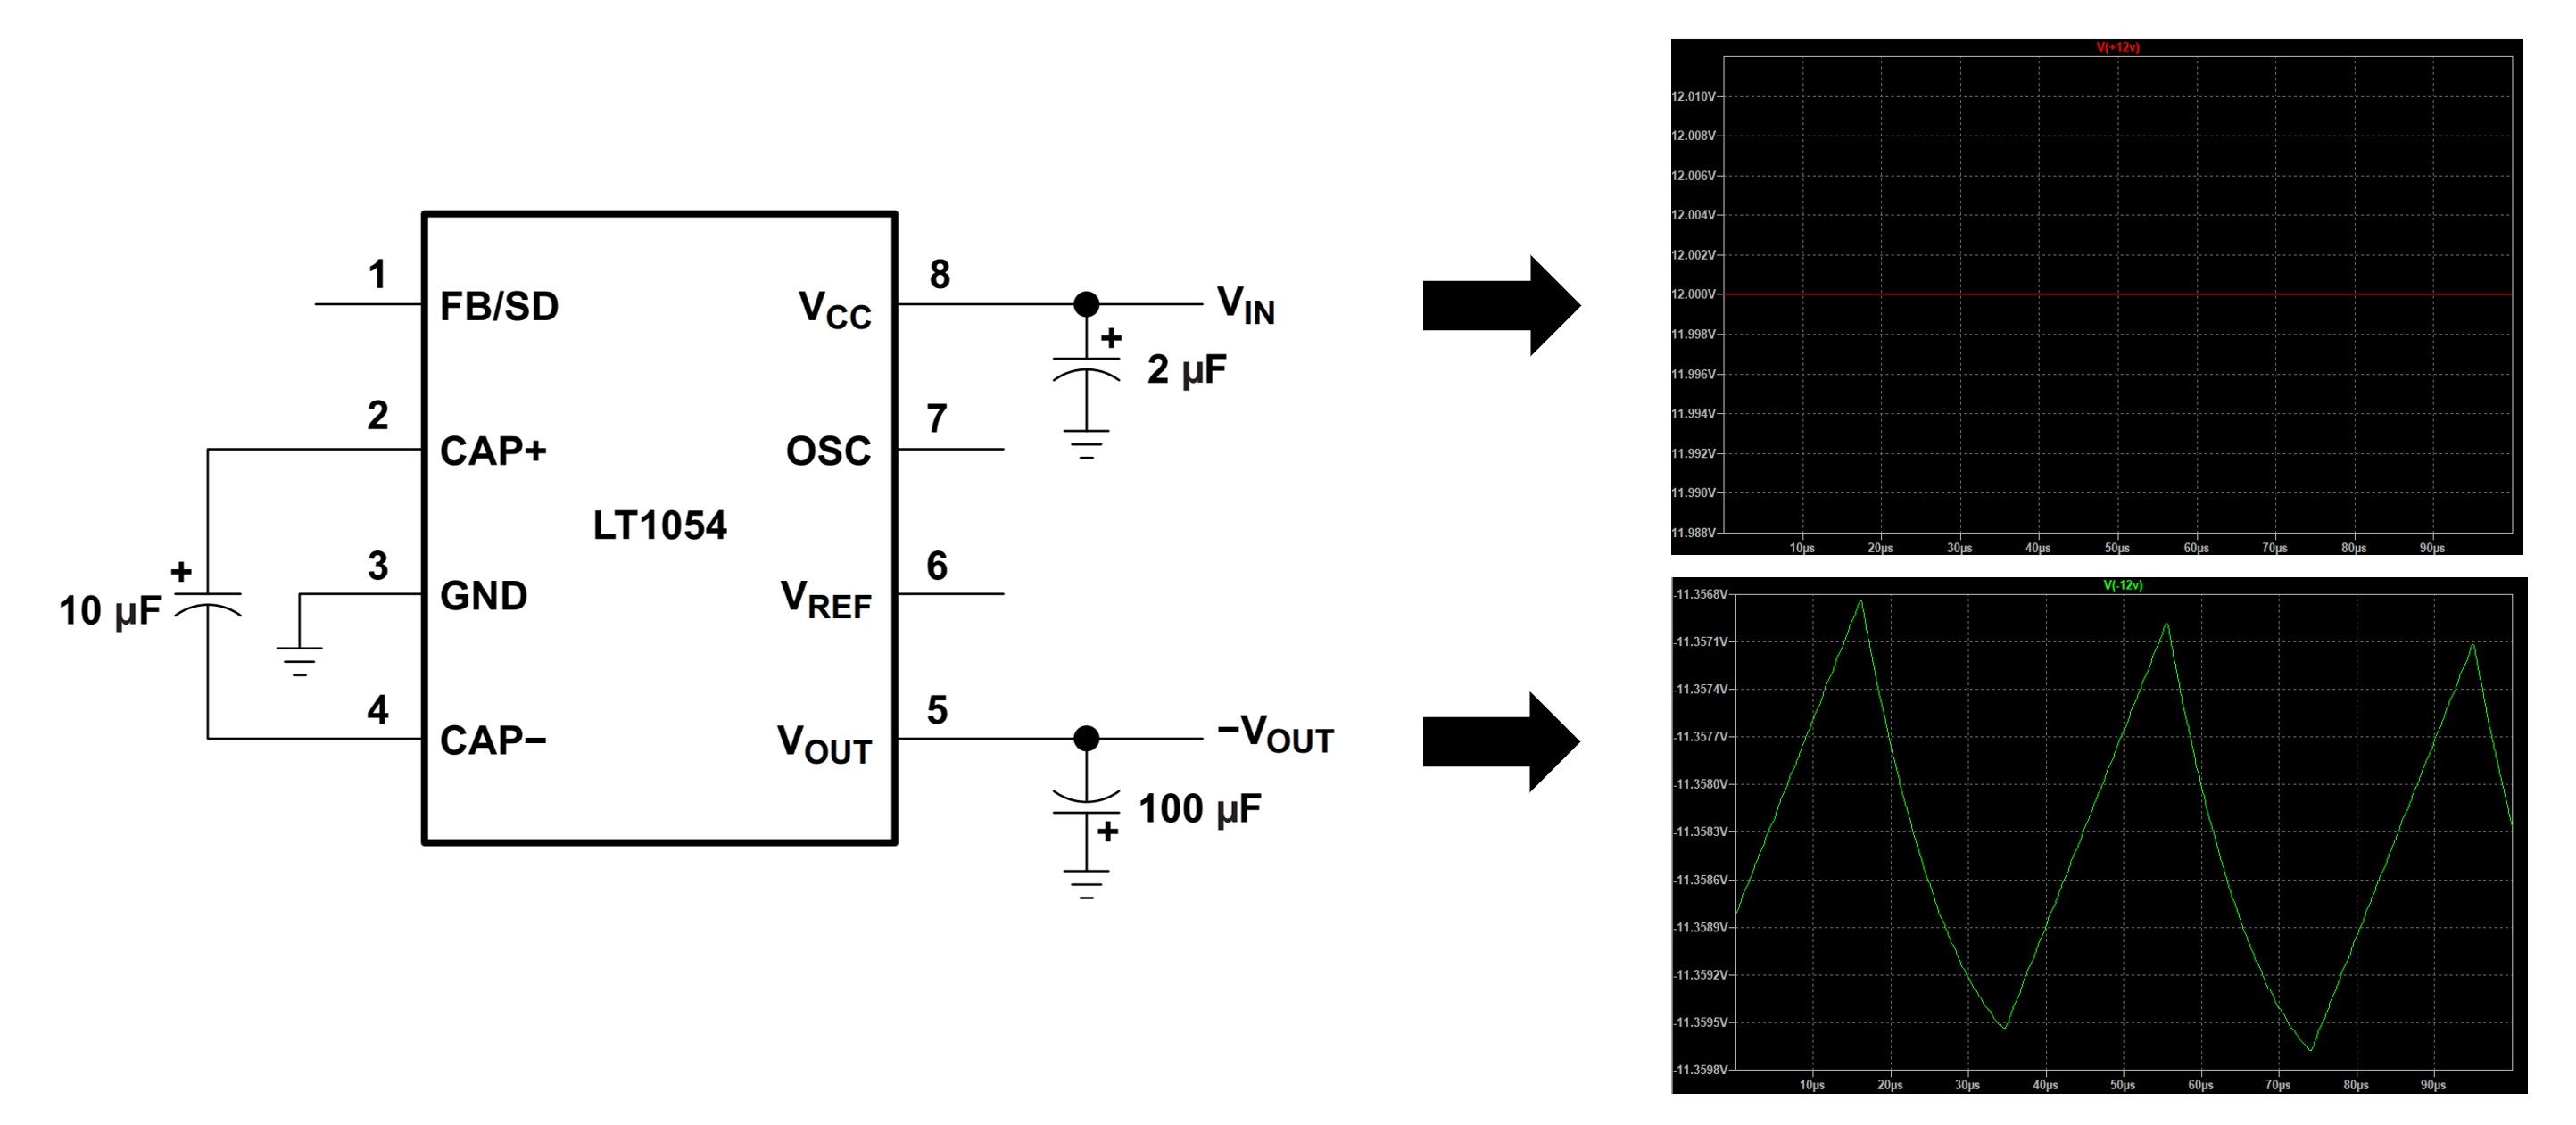
\includegraphics[width=0.6 \textwidth]{DCDC.jpg}
	\caption[Beschaltung und erzeugte Spannung des LT1054]{Beschaltung und erzeugte Spannung des LT1054} 
	\cite{LT1054} \cite{Eigene Darstellung}
	\label{fig:DCDC}
\end{figure}

Der Spannungswandler arbeitet außerdem intern für die Invertierung mit einer Nennfrequenz von 25kHz. Da die zu übertragenden Daten auch nahe diesem Bereich liegen, empfiehlt es sich den Pfad der Signalverarbeitung und den der Spannungsinvertierung auf der Platine möglichst weit auseinander zu platzieren um möglichen Parasitären Störungen vorzubeugen.


\subsection{Arduino UNO V3}
\label{subsec:Unterabschnitt12}

Die Arduino-Plattform besteht prinzipiell aus der auf C und C++ basierenden Entwicklungsumgebung und der zu Programmierenden Hardware\gls{online:arduino}. Vorteilhaft ist hier die gute Dokumentation und eine große menge an Bibliotheken zum einbinden externer Hardwarekomponenten. Ein zusätzlicher Vorteil der Plattform liegt in ihrer Quelloffenheit. Alle zugehörigen Komponenten sind demnach 'Open Source'. Das hat zur Folge, dass Codes der Bibliotheken und des Bootloaders frei zur Verfügung stehen und nach belieben verändert werden können. Auch die Architektur der Hardware ist offengelegt, weshalb Hersteller eigene kompatible Boards konstruieren und verkaufen können. Durch die Unabhängigkeit von Programmierer und Hersteller entsteht eine erschwingliche Hardware, welche bezüglich der Quelloffenheit ohne Einschränkungen programmiert werden kann.[10 - Evans, Beginning Arduino Programming. Apress, 2011, ISBN: 978-1-4302-3777-8]Diese eignet sich hervorragend zur Funktionsprogrammierung von ansteuerbaren Komponenten im Analogen Signalverarbeitungspfad.

\section{Verwendete Tools}       
\subsection{LT-Spice}
\label{subsec:Unterabschnitt12}
LT-Spice ist eine SPICE-basierte Computersoftware zur Simulation analoger elektronischer Schaltungen. Diese wurde vom Halbleiterhersteller Analog Devices (ursprünglich von Linear Technology) entwickelt. Es ist die am weitesten verbreitete und verwendete SPICE-Software in der Elektro-Simulationsbranche. Obwohl es sich um freie Software handelt, ist LT-Spice nicht künstlich eingeschränkt, um seine Funktionalität einzuschränken.\gls{online:spice} Diese Simulationssoftware würde im Rahmen dieser Arbeit zur Erprobung und Simulation des analogen Signalverarbeitungsschaltkreises verwendet.

\subsection{Eagle}
\label{subsec:Unterabschnitt12}

EAGLE ist eine Software zum designen und erstellen von Leiterplattenlayouts. Die Software verfügt über einen Schaltplan- und einen Layouteditor, sowie über eine sehr umfassende Bibliothek an Bauteilen, welche sehr unkompliziert und individuell erweiterbar ist.\gls{online:eagle1}\gls{online:eagle2}

\subsection{Arduino \gls{acr:IDE}}
\label{subsec:Unterabschnitt12}

Die Sprachen welche in der Entwicklungsumgebung genutzt werden sind C und in kleineren Umfängen auch C++. In den Standardbibliotheken der Entwicklungsumgebung sind die für die Programmierung erheblichsten Funktionen zusammengefasst. Um ein weitere Funktionen zu nutzen, können dementsprechend zusätzliche Bibliotheken eingebunden werden. 
Der Editor mit integriertem Compiler ist ein weiterer Bestandteil der \gls{acr:IDE}. In diesem wird der Code geschrieben, kompiliert und auf das Board überspielt. User benötigen also nur eine Software, um ihre Mikrocontroller in vollen Umfängen nutzen zu können. Dieses \gls{acr:IDE} bietet außerdem die Möglichkeit, Bibliotheken oder gar Programmbeispiele herunterzuladen. 

[10B. Evans, Beginning Arduino Programming. Apress, 2011, ISBN: 978-1-4302-
3777-8.].

\begin{figure}[H]
	\centering
	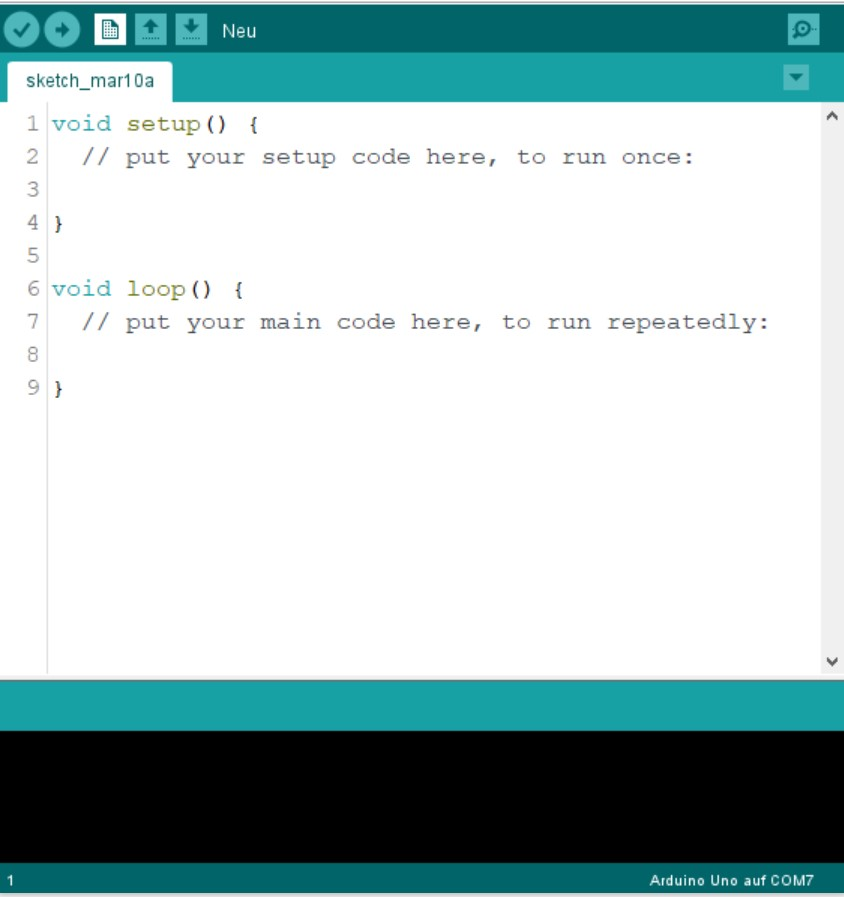
\includegraphics[width = 0.6 \textwidth ]{ide.jpg}
	\caption[Arduino \gls{acr:IDE}]{Arduino \gls{acr:IDE}}\gls{online:Eigen}
	\label{fig:ide}
\end{figure}


Arduino-Programme basieren immer auf einem einheitlichen Grundaufbau. In Abb. ist
dieser zu erkennen. Es sind zwei Funktionen namens setup() und loop() deklariert.
Setup() wird einmalig zu beginn des Programms aufgerufen, während loop() direkt im Anschuss aufgerufen wird, bis der Mikrocontroller stromlos geschaltet wird. Oberhalb der Funktion setup() können außerdem noch Präprozessorbefehle programmiert werden.

\subsection{Dream}
\label{subsec:Unterabschnitt12}
Die Software Dream bietet eine alternative Radiosignale auf dem Computer zu empfangen und auch zu senden. Sie war ursprünglich als Forschungsprojekt des Fraunhofer Instituts angesetzt. Signale welche nicht über den PC empfangen werden können, werden über den Mikrofoneingang der Soundkarte empfangen.
Bei alldem benutzt das Konzept internationale Direktiven für Amateurfunk, Radio und Informationsdienste.
Diese Eigenschaft ermöglicht es dem User FM, AM und \gls{acr:DRM} zu empfangen. Außerdem visualisiert die Software in Echtzeit zahlreiche Daten, Statistiken und Diagramme des empfangenen Signals. \gls{online:dream} Die Modulation und das Senden des OFDM-Signals über die konstruierte Hardware erfolgt durch diese Software und wird in folgenden Kapiteln noch weiter intensiviert.